\documentclass[11pt,a4paper]{article}
\usepackage[utf8]{inputenc}
\usepackage[T1]{fontenc}
\usepackage{lmodern}
\usepackage[margin=25mm]{geometry}
\usepackage{amsmath,amssymb,booktabs,array,graphicx,microtype}
\usepackage[numbers,sort&compress]{natbib}
\usepackage[hidelinks]{hyperref}
\usepackage{xcolor}
\newcommand{\pending}[1]{\par\noindent\textcolor{blue!60!black}{\textbf{Results pending.} #1}\par}
\newcommand{\asset}[3]{\begin{figure}[htbp]\centering
  \IfFileExists{#1}{\includegraphics[width=.94\linewidth]{#1}}
  {\fbox{\parbox{.88\linewidth}{\centering\textbf{Figure not yet produced.}\\\small\path{#1}}}}
  \caption{#2}\label{#3}\end{figure}}
\newcommand{\tablepath}[1]{\par\noindent\textit{Machine-readable table to populate this result:} \path{#1}.\par}
\newcommand{\draftstatus}{\begin{center}\small\textbf{Substantive research draft---5 November 2026.}\\
  Numerical results under this protocol have not been produced or validated for this draft.
  Code execution, statistical checks and \LaTeX{} compilation remain to be performed.\end{center}}
\newcommand{\R}{\mathbb{R}}
\newcommand{\ind}{\mathbf{1}}
\author{Th\'eotime Coudray, St\'ephane Goutte}
\date{5 November 2026}

\date{12 November 2026}
\title{Criticality Indicators for Deadline-Constrained Energy Optimization:\\
Physical Descriptors, Predictive Validation and Preference-Dependent Weights}
\begin{document}
\maketitle
\begin{abstract}
Energy-system optimization must deliver useful dispatches within operational
deadlines. We examine a 22-component criticality indicator on 600 constructed
scenarios, separating generator parameters, realized MILP data and descriptive
proxies. Nested scenario-grouped validation evaluates economic and joint
economic--service success under five independent deadlines from 5 to 120 seconds.
The original scalar adds information beyond size in seven of ten historical
endpoint--deadline comparisons, while separate components improve prediction.
For five operational preferences, a new intermediate model separates a common
nonnegative weight direction from deadline-specific amplitudes. Rescaling the
common direction reduces mean squared error by 11.9--40.0\%; separate directions
reduce it by another 24.3--36.1\%. Twenty-three of 25 direction contrasts retain
positive lower bounds in simultaneous intervals over the 50 primary contrasts.
However, leaving a complete family out increases this linear model's pooled
MSE by factors of 2.72--3.63. An audit identifies an almost duplicated demand
proxy, and reduced representations retain similar predictive performance.
Within held-out portfolios, adaptive time allocation improves observed joint
success over uniform allocation: 415 versus 341 successes at 30 seconds reserved
per scenario on average. A three-component allocation performs similarly,
showing that decision utility need not require the richest predictor.
A historical exploratory follow-up recomputes descriptors on constructed
MILPs and identifies extreme affine extrapolation of the line-to-zone ratio.
A positive fractional-logistic model without that coordinate reduces MSE
by 19.1--30.6\% under scenario folds and 38.1--60.8\% under family holdout,
relative to the realized-descriptor linear predictor projected onto $[0,1]$.
These post-hoc findings remain development evidence. The independent
400-scenario campaign is in progress; its predictors were frozen before
execution and have not been replaced by the exploratory bounded models.
No independent-test performance estimate is reported here.
\end{abstract}

\section{Introduction}
Increasing shares of variable renewable generation change both the magnitude
and temporal structure of the flexibility required to operate power systems.
Generation, storage, demand response and interconnections provide different
combinations of power, energy and ramping capability. Flexibility assessment
therefore depends on the relationship between these resources and the
variations they must accommodate \citep{lannoye2012,ulbig2015}. Operational
optimization translates these physical capabilities into coordinated decisions
while balancing economic and service requirements.

Mixed-integer linear programming (MILP) provides a framework for representing
commitment decisions together with continuous dispatch and intertemporal
constraints. Research on unit commitment shows that formulation strength and
compactness affect computational performance \citep{moralesespana2013}.
Physical stress and computational difficulty consequently need not coincide:
a system with little flexibility may admit few operating choices, whereas a
system with substantial capacity may present many competing commitment and
storage schedules. System size alone is also an incomplete description of
this distinction.

For an operational decision, the relevant outcome is the delivery of a
physically valid and sufficiently useful dispatch before a deadline. A
feasible dispatch may still contain unserved energy, and an economically
acceptable dispatch need not have low emissions. Conversely, an operationally
useful solution need not be accompanied by a proof of global optimality.
Characterizing difficulty thus requires an explicit outcome, an optimization
method and a resource allocation. This perspective connects energy-system
assessment to empirical models of algorithm performance, which relate
instance features to observed computational outcomes \citep{hutter2013}.

A composite criticality indicator offers a compact way to combine physical
stress and structural descriptors before optimization. Its interpretation,
however, depends on normalization, correlated components and aggregation
weights. These are substantive methodological choices in composite-indicator
construction \citep{oecd2008}. Equal weighting is a transparent reference
convention, but does not demonstrate equal predictive contributions. Likewise,
a component that strongly changes the arithmetic score may add little
information about operational outcomes once related descriptors are known.
Predictive validation and arithmetic sensitivity therefore answer distinct
questions.

This study examines that distinction and estimates component weights for
explicit operational preferences. First, we define a 22-component indicator
and quantify how its aggregation affects scenario rankings. Second, we test
whether the indicator and its decomposition predict timely economic and
service success beyond system size. Third, we learn nonnegative weights for
five targets combining unserved energy, cost, execution time and direct
thermal CO$_2$ intensity, comparing a common coefficient vector with separate
vectors for each deadline, including a shared-direction intermediate
model. We then test transfer between families and the utility of time
allocation within held-out portfolios. Scenario-grouped nested validation separates
parameter estimation from predictive assessment; interpretation remains
conditional on the deliberately constructed sampling regimes.
An explicitly exploratory follow-up then recomputes descriptors on the
constructed MILP and compares projected linear prediction, bounded regression
and removal of the line-to-zone coordinate. Its historical evidence and the
ongoing independent campaign are reported as separate stages.

The contribution is an empirical assessment of interpretable criticality
representations and their preference dependence. It also establishes the
starting point for subsequent work on method complementarity: if
scenario descriptors anticipate the difficulty faced by one method, do
different optimization methods deliver complementary combinations of time,
cost and service on those scenarios? This distinction follows the broader
algorithm-selection framework \citep{rice1976,xu2008,bischl2016}, but predictive
accuracy alone cannot establish a useful selection policy.

\begin{table}[htbp]\centering\small
\begin{tabular}{>{\raggedright\arraybackslash}p{.23\linewidth}>{\raggedright\arraybackslash}p{.31\linewidth}>{\raggedright\arraybackslash}p{.35\linewidth}}\toprule
Research strand & Object being measured & Relation to this study\\\midrule
Physical flexibility \citep{lannoye2012,ulbig2015,terca2026flexibility} & Ability to accommodate residual-load variation over time & Physical descriptors do not by themselves measure algorithm runtime\\
Empirical algorithm performance \citep{hutter2013} & Outcome of a specified method on an instance & Delivery, economic quality and service are explicit endpoints\\
Composite indicators \citep{oecd2008} & Aggregation under normalization and weighting conventions & Arithmetic sensitivity is separated from predictive weight estimation\\
Selection and resource allocation \citep{rice1976,bischl2016} & Decisions improving a portfolio's outcomes & The present decision experiment allocates time to HiGHS; cross-method selection is distinct\\\bottomrule
\end{tabular}
\caption{Positioning: physical adequacy, computational prediction, aggregation and decisions answer different questions.}
\end{table}
Feature-based benchmark selection, as used by MIPLIB \citep{miplibselection},
also makes the sampling design an explicit part of evaluation. General MIP
instances cannot directly replace energy scenarios requiring these physical
descriptors. PGLib-UC \citep{pglibuc} offers a complementary unit-commitment
benchmark, but its system-wide demand formulation does not reproduce every
multizone storage and load-shifting component studied here; an external
adapter would need to identify the common formulation and unavailable features.

\section{Methods}
\label{sec:methods}
\subsection{What constitutes one scenario?}
\label{sec:scenario_definition}
A scenario is one fully specified deterministic energy-system instance,
not one solver execution and not one stochastic realization inside a
stochastic-programming model. Write
\begin{equation}
 s=(\mathcal Z,\mathcal T,\Delta t,\mathcal L,
     D,\overline P^{\rm ren},I^{\rm hydro},\mathcal K,
     \mathcal X_0,\mathcal X_T,\mathcal C),
 \label{eq:scenario_tuple}
\end{equation}
where the entries specify zones, time steps, time-step duration, transport
lines, demand, renewable availability, hydro inflows, installed capacities
and operating limits, initial states, terminal requirements, and costs.
These data are fixed before optimization. The MILP chooses dispatch and
operating modes; it does not choose the installed equipment or the demand
profile. Every deadline and repetition associated with $s$ uses the same
physical instance. Changing only the computational deadline creates a new
execution of the same scenario, not a new independent scenario.

Three layers must be distinguished. A generator first samples parameters
such as equipment counts, demand scale and weather categories. A deterministic
loader, seeded by the scenario identifier, converts these parameters into
zone--time arrays and operating limits. Finally, the historical criticality calculation
maps the generator metadata into 22 descriptors. Those descriptors are
coarse summaries of the instance, not the MILP input vector itself; several
use nominal approximations rather than the realized time series. The separate
realized-descriptor follow-up is defined in Section~\ref{sec:bounded_method}.

\begin{table}[htbp]\centering\small
\begin{tabular}{>{\raggedright\arraybackslash}p{.19\linewidth}>{\raggedright\arraybackslash}p{.37\linewidth}>{\raggedright\arraybackslash}p{.33\linewidth}}\toprule
Scenario dimension & What varies between scenarios & Effect in the realized MILP\\\midrule
Spatial structure & Region and zone counts; regional equipment allocation & 4--170 zones; one aggregated dispatch model per zone\\
Demand and weather & Demand category and multiplier (0.701--1.699); weather categories, local profile mixtures and perturbations & Fixed demand, solar/wind availability and hydro-inflow arrays\\
Generation & Thermal, nuclear, solar, wind and hydro equipment counts; thermal ramp fraction (0.204--0.949) & Capacities, minima, ramp limits and variable/start-up costs; thermal commitment is aggregated by zone\\
Storage & Battery/pumped counts, efficiencies, retention, initial/terminal levels; a separate nominal duration proxy & Charge/discharge limits and energy balances; installed historical batteries use the loader's fixed 4-hour duration\\
Demand response & Equipment counts and maximum deferred share (0.050--0.300) & Deferral/recovery capacities, cost blocks, active-period and ramp limits\\
Exchange & Intertie parameter (0.150--0.799), neighbour count, trade policy and cap factor & Line capacities and import/export limits; realized historical networks remain trees\\
Economics & Fuel, start-up, cycling and spill costs; carbon price (35.15--218.83 EUR/t); ENS penalty (6015--39787 EUR/MWh) & Coefficients of the validated dispatch objective\\
Time and physics & Fixed in the historical cohort: 24 hourly steps; common equations and tolerances & Temporal resolution and transport physics do not vary in the 600 cases\\\bottomrule
\end{tabular}
\caption{Scenario inputs and their role. Numeric intervals are observed minima and maxima in the selected 600 scenarios, rounded for readability; they are not uniform sampling bounds. The released parameter table gives all values by scenario and family.}
\label{tab:scenario_parameters}
\end{table}

The generator's continuous and integer draws are uniform within declared
family-specific ranges, while categorical choices and regional allocations
have their own rules. Criticality-based selection then changes their joint
distribution. In particular, the intertie parameter changes line capacities
and nominal distances, but the historical loader constructs within-region
chains joined between neighbouring regions, giving $|\mathcal L|=|\mathcal Z|-1$.
It does not independently sample mesh density. Installed units are aggregated
within each zone: increasing a thermal equipment count changes capacity,
not the number of zone-level commitment variables. Appendix~\ref{app:milp}
gives the optimization variables and equations, including the distinction
between metadata and implemented constraints.

\subsection{Energy-system model and operational outcomes}
The physical model coordinates thermal and nuclear generation, renewable
curtailment, batteries, reservoir and pumped hydro, demand response,
interzonal flows and external trade. Its objective includes operating and
start-up costs, flexibility activation, storage cycling, curtailment,
unserved energy and overgeneration penalties. Thermal commitment satisfies
transition equations, initial conditions and operating, start-up and shutdown
ramp limits. Demand response is represented as lossless load shifting with
a causal energy backlog and terminal repayment. Storage balances account
for efficiencies, retention and terminal conditions. Interzonal exchange
uses a capacitated transport model; Kirchhoff's laws and security constraints
are outside the formulation.

A dispatch is checked independently of the solver's reported objective and
residuals. Validation reconstructs costs and physical balances and checks
integrality, commitment transitions, ramps, storage, demand-response
repayment, exchange limits and nodal balances. The absolute physical and
integrality tolerances are $10^{-3}$ and $10^{-5}$, respectively. Since
unserved energy is permitted as a penalized action, physical validity and
service continuity are assessed separately.

For scenario $s$ and independently allocated deadline $b$, let $F_{sb}=1$
if a valid dispatch is delivered and the complete execution terminates
within $b$. Elapsed time includes scenario processing, model construction,
optimization, validation and delivery of the result; static library and
model preload is excluded. A feasible incumbent available only within an
unfinished or late execution does not satisfy this condition. Let $C_{sb}$
be the validated operating objective and $C_s^{\rm ref}$ a common reference
cost. For $|C_s^{\rm ref}|>1$ euro, define
\begin{equation}
 g_{sb}^{\rm ref}=\frac{C_{sb}-C_s^{\rm ref}}{|C_s^{\rm ref}|},\qquad
 Q_{sb}=\ind\{g_{sb}^{\rm ref}\leq0.05\}.
 \label{eq:economic}
\end{equation}
Negative gaps are retained when a dispatch improves the reference incumbent.
For $|C_s^{\rm ref}|\leq1$ euro, the quality criterion instead requires
$C_{sb}-C_s^{\rm ref}\leq1$ euro. With unserved energy $E_{sb}$ in MWh, the
two binary outcomes are
\begin{equation}
 Y^{\rm E}_{sb}=F_{sb}Q_{sb},\qquad
 Y^{\rm ES}_{sb}=F_{sb}Q_{sb}\ind\{E_{sb}\leq10^{-3}\ \mathrm{MWh}\}.
 \label{eq:binary_endpoints}
\end{equation}
E denotes economic success and ES joint economic--service success.
An observed execution failure has outcome zero. An unexecuted trial or
missing information required to assess an otherwise delivered dispatch
remains unknown.

\subsection{Physical and structural components of criticality}
\label{sec:components}
The indicator combines a physical-stress block $\mathcal A$ of twelve
components and a computational-structure block $\mathcal B$ of ten
components. All descriptors are available before optimization. They
summarize scenario parameters and resource configurations rather than
post-optimization trajectories. Several are deliberately coarse proxies;
their physical interpretation does not imply that they measure realized
stress or actual search complexity exactly.

Let $N$ be the zone count, $N_T$ the time-step count, $T_h$ the horizon in
hours, and $n_{\rm th}$ and $n_{\rm nu}$ the thermal and nuclear equipment
counts. The descriptors use nominal capacities of 300~MW per thermal unit
and 1000~MW per nuclear unit. For demand multiplier $d$ and renewable
penetration $v$, define the approximations
\begin{align}
 \widehat P_D&=500N d, & \widehat P_{\rm peak}&=1.3\widehat P_D, &
 \widehat P_F&=300n_{\rm th}+1000n_{\rm nu},\nonumber\\
 \widehat R&=\widehat P_{\rm peak}(1-0.3v), &
 \widehat E_R&=0.4T_h\widehat R, &
 \widehat D&=T_h\widehat P_D.
 \label{eq:descriptor_approximations}
\end{align}
These quantities construct the descriptors; dispatch and service outcomes
use the realized physical data. Denote total storage power and energy by
$P_{\rm st}$ and $E_{\rm st}$, demand-response power by $P_{\rm DR}$,
fractional thermal ramp capability by $r_{\rm th}$ and intertie density by
$\rho$. Adequacy ratios use a positive denominator floor of 1 in the
corresponding unit. A7--A9 are clipped to $[-1,1]$, and A10 to $[0,1]$,
before normalization.

\begin{table}[htbp]\centering\small
\begin{tabular}{lp{.59\linewidth}rr}\toprule
ID & Raw definition or interpretation & $\ell_j$ & $u_j$\\\midrule
A1 & Renewable penetration $v$ & 0 & 1.5\\
A2 & Generator volatility proxy $\mathrm{round}(\sqrt{v_W^2+v_D^2},3)$ & 0 & 0.5\\
A3 & Demand-scale-derived proxy $\mathrm{round}(1.8d,2)$ & 1 & 10\\
A4 & Short-term variability coefficient of the weather regime & 0 & 0.3\\
A5 & Demand multiplier $d$ & 0.5 & 2\\
A6 & Peak-to-firm ratio $\widehat P_{\rm peak}/\widehat P_F$ & 0.3 & 1.5\\
A7 & Inverse storage-power adequacy $1-P_{\rm st}/\widehat R$ & $-1$ & 1\\
A8 & Inverse storage-energy adequacy $1-E_{\rm st}/\widehat E_R$ & $-1$ & 1\\
A9 & Inverse thermal flexibility $1-300n_{\rm th}r_{\rm th}/\widehat R$ & $-1$ & 1\\
A10 & Inverse demand-response headroom $1-P_{\rm DR}T_h/\widehat D$ & 0.5 & 1\\
A11 & Trade-exposure coefficient times $\min(n_{\rm neighbours}/4,1)$ & 0 & 0.5\\
A12 & Inverse intertie-density proxy $1-\rho$ & $-1$ & 1\\\bottomrule
\end{tabular}
\caption{Physical-stress components and fixed normalization bounds.
All quantities describe the scenario before optimization.}
\label{tab:components}
\end{table}

A4 assigns coefficients 0.08, 0.22, 0.18, 0.06 and 0.14 to calm winter,
stormy winter, sunny summer, overcast summer and mixed weather, respectively.
A11 uses trade-exposure coefficients 0.25, 0.15 and 0.02 for unrestricted,
capped and blocked trade. These mappings are fixed descriptive conventions;
they are not estimated from the operational outcomes.
For A2, weather coefficients $v_W$ are 0.12, 0.25, 0.22, 0.10 and 0.18
in the same weather order as A4; demand-category coefficients $v_D$ are
0.15, 0.08, 0.20, 0.22 and 0.10 for weekday peak, weekend flat, cold snap,
heatwave and shoulder profiles. A3 is not the ratio of realized maximum to
minimum demand: the code audit reconstructs all 600 stored values exactly
as $\mathrm{round}(1.8d,2)$. A true peak-to-valley ratio is invariant to
uniform demand scaling. This definitional correction preserves the historical
values and explains their near-perfect correlation with A5.

The structural block describes scale, commitment, intertemporal restrictions
and network organization (Table~\ref{tab:structural_components}). B3 is an
estimate associated with scenario construction, rather than a count of free
integer decisions in the realized formulation. B9 represents regional
connectivity potential rather than realized line count. These distinctions
matter when interpreting topology or formulation changes.

\begin{table}[htbp]\centering\small
\begin{tabular}{lp{.59\linewidth}rr}\toprule
ID & Raw definition or interpretation & $\ell_j$ & $u_j$\\\midrule
B1 & Zone count $N$ & 4 & 400\\
B2 & Time-step count $N_T$ & 12 & 168\\
B3 & Generator estimate $N_T(2n_{\rm th}+2n_{\rm nu}+3N+1)$ & 500 & 50000\\
B4 & Thermal equipment density $n_{\rm th}/N$ & 0 & 3\\
B5 & Minimum-generation ratio proxy, fixed at 0.35 & 0.1 & 0.6\\
B6 & Start-up cost relative to estimated horizon variable cost & 0 & 0.5\\
B7 & Ramp tightness $300n_{\rm th}/\max(300n_{\rm th}r_{\rm th},1)$ & 0.5 & 10\\
B8 & Storage duration divided by terminal state-of-charge tolerance & 0.1 & 100\\
B9 & $\rho R_g(R_g-1)/(2N)$, where $R_g$ is region count & 0.1 & 2\\
B10 & Coefficient of variation of zone counts across regions & 0 & 1\\\bottomrule
\end{tabular}
\caption{Computational-structure proxies and fixed normalization bounds.}
\label{tab:structural_components}
\end{table}

For B6, estimated horizon variable cost is
$0.5T_h(300n_{\rm th}+1000n_{\rm nu})c_{\rm fuel}$, where $c_{\rm fuel}$
is thermal fuel cost per MWh. Total start-up cost sums thermal and nuclear
equipment contributions; the ratio is capped at 0.5 and its denominator
floored at one euro. For B8, terminal tolerance is floored at 0.01. B10 is
zero for a single region and otherwise divides the population standard
deviation of regional zone counts by their mean, floored at one. The
constant B5 cannot explain differences among scenarios. Horizon effects
are similarly unidentifiable in a fixed-horizon cohort.

\subsection{Reference aggregation and arithmetic sensitivity}
\label{sec:score_sensitivity}
For raw component $x_{sj}$, fixed bounds $\ell_j<u_j$ define
\begin{equation}
 z_{sj}=\min\{1,\max\{0,(x_{sj}-\ell_j)/(u_j-\ell_j)\}\}.
 \label{eq:normalization}
\end{equation}
Bounds are fixed before predictive fitting and are not adapted to validation
observations. The reference indicator assigns equal weights within each
block and equal weight to the two blocks:
\begin{equation}
 S_s=\frac1{12}\sum_{j\in\mathcal A}z_{sj},\qquad
 H_s=\frac1{10}\sum_{j\in\mathcal B}z_{sj},\qquad
 I_s=\tfrac12 S_s+\tfrac12 H_s.
 \label{eq:reference_index}
\end{equation}
Each physical component has weight $1/24$ and each structural component
weight $1/20$. This convention differs from equal weighting of all 22
components and from the equal-priority operational target introduced below.
More generally, with nonnegative within-block weights summing to one,
\begin{equation}
 I_\theta(s)=\lambda S_w(s)+(1-\lambda)H_w(s),\quad
 S_w=\sum_{j\in\mathcal A}w^A_jz_{sj},\quad
 H_w=\sum_{j\in\mathcal B}w^B_jz_{sj},\quad 0\leq\lambda\leq1.
 \label{eq:weighted_index}
\end{equation}
Changing these weights changes the description and ordering of scenarios;
it does not change their physical problems or observed dispatches. For
fixed normalized components, away from clipping boundaries,
\begin{equation}
 \frac{\partial I_\theta}{\partial\lambda}=S_w-H_w,\qquad
 \frac{\partial I_\theta}{\partial x_j}
 =\frac{c_j}{u_j-\ell_j}\ind\{\ell_j<x_j<u_j\},
 \label{eq:raw_sensitivity}
\end{equation}
where $c_j=\lambda w_j^A$ or $(1-\lambda)w_j^B$. Sensitivity depends jointly
on weighting and normalization; saturation removes sensitivity to further
raw extremes. A within-block weight transfer $\delta$ from $k$ to $j$
changes the stress contribution by $\lambda\delta(z_j-z_k)$. Removing a
constant component and renormalizing can change the balance between blocks
even though the component contains no ranking information.

The descriptive analysis varies $\lambda$ over $\{0,0.25,0.5,0.75,1\}$ and
removes each component in turn, renormalizing within its block. It assesses
absolute score changes, Spearman rank correlation, pair reversals and
migration across intervals of width 0.2. Comparisons use unrounded component
sums and the reference bounds. These diagnostics are separate from
predictive model selection. The identity
$\operatorname{Var}(I)=\boldsymbol c^\top\Sigma_z\boldsymbol c$ includes
covariances: arithmetic contributions cannot be interpreted as unique
predictive or causal effects.

\subsection{Regression models for economic and service success}
\label{sec:binary_models}
The first analysis estimates success probabilities using regularized
logistic regression, separately for each deadline and endpoint:
\begin{equation}
 \widehat p(Y_{sb}=1\mid X_s,b)
 =\operatorname{logit}^{-1}(a_b+\boldsymbol\beta_b^\top X_s).
\end{equation}
The size baseline contains zone count, time-step count, line count and the
zone--time product. We compare additions of the scalar $I$, the two blocks
$(S,H)$, six interpretable components, and all 22 components. The
six-component subset comprises A2, A6, A8, A10, B3 and B7: residual
volatility, firm-capacity stress, storage-energy adequacy, demand-response
headroom, estimated combinatorial load and ramp tightness. No cost,
incumbent, solver bound or other post-optimization quantity is a predictor.

Two versions of each model distinguish pooled information beyond size from
refinement conditional on the known sampling family. Family membership
encodes a targeted parameter regime and criticality-based selection; it is
not independent of the indicator's inputs. A small gain after conditioning
on family measures limited residual refinement rather than total predictive
information in the pooled cohort.

To distinguish interactions from nonlinear individual associations, further
models use the fixed additive basis
$h(z)=(z,(z-0.25)_+,(z-0.75)_+)$, followed by five centered products:
A2$\times$A8, A2$\times$B7, A6$\times$A10, A8$\times$B8 and B3$\times$B9.
These pairs examine whether associations of variability and adequacy with
success depend on storage, ramping, demand response or network structure.
Both parent main effects are retained for every product. Writing
$\mathcal P$ for the pairs, the model is
\begin{equation}
 \begin{aligned}
 \operatorname{logit}\widehat p_{sb}
 &=a_b+\boldsymbol\gamma_b^\top X_s^{\rm size}
 +\eta_{b,\mathrm{family}(s)}+\sum_j g_{jb}(z_{sj})\\
 &\quad+\sum_{(j,k)\in\mathcal P}\theta_{jk,b}
 (z_{sj}-\mu_j)(z_{sk}-\mu_k).
 \end{aligned}
 \label{eq:targeted_interactions}
\end{equation}
The family term is omitted in pooled models. Training observations alone
define centering means $\mu_j$, imputation and feature scaling. Constant
parents make their products unidentifiable. This comparison concerns
interaction on the log-odds scale, conditional on the specified main effects.

Component contribution is evaluated by refitting after removal of its
linear, nonlinear and associated product terms. The targeted set is A2,
A6, A8, A10, B3, B7, B8 and B9. Pair removal deletes only that product.
Loss differences quantify conditional information under the fitted model
class; correlated components can substitute for each other, so these
contrasts do not define weights for the scalar indicator \citep{fisher2019}.

\subsection{Supervised weights for a joint operational loss}
\label{sec:p1_weight_method}
The second analysis estimates component weights directly for five
explicit operational preferences. It uses the same 600 scenarios and five
independent HiGHS runs per scenario (primary repetition), without family
indicators or interaction terms. Execution times are never added across
budgets. Each observation retains its own deadline $b$ and process-exit
measurement $t^{\mathrm{exit}}_{sb}$.

For a valid dispatch delivered within $b$, let $D_s$ denote total demand
in MWh, $E_{sb}$ unserved energy in MWh, $C_{sb}$ operating cost, and
$C_s^{\mathrm{ref}}$ the historical reference cost. Define
\begin{equation}
\begin{aligned}
 h(x;a)&=\frac{x}{x+a},\qquad
 T_{sb}=\frac{t^{\mathrm{exit}}_{sb}}{b},\\
 e_{sb}&=\frac{\max(E_{sb}-0.001,0)}{D_s},\qquad
 g_{sb}=\max\!\left(\frac{C_{sb}-C_s^{\mathrm{ref}}}
 {\max(|C_s^{\mathrm{ref}}|,1\ \mathrm{EUR})},0\right),\\
 Q^{\mathrm{CO2}}_{sb}&=\begin{cases}
 h\!\left(\dfrac{0.72\sum_{z,t}p^{\mathrm{thermal}}_{sbtz}\Delta t}
 {D_s-\max(E_{sb},0)};0.72\right),&D_s-\max(E_{sb},0)>10^{-12},\\
 1,&D_s-\max(E_{sb},0)\leq10^{-12},
 \end{cases}\\
 Y^{(p)}_{sb}&=\pi^{(p)}_E h(e_{sb};0.01)
 +\pi^{(p)}_C h(g_{sb};0.05)+\pi^{(p)}_T T_{sb}
 +\pi^{(p)}_Q Q^{\mathrm{CO2}}_{sb}.
\end{aligned}
\label{eq:p1_joint_loss}
\end{equation}
The thermal emissions factor is 0.72~tCO$_2$/MWh; the intensity inside $h$
is measured in tCO$_2$ per served MWh. The carbon term is set to one when served energy
is at most $10^{-12}$~MWh. Non-delivery or invalid output receives
$Y^{(p)}_{sb}=1$ for every preference; missing ENS and emissions remain
unknown rather than being recorded as zero. Lower targets are better.
Thus the response is a joint operational nonperformance score, not time
to optimality, a pure emissions measure, or a sum of solve times.
The transformation $h(x;a)$ maps a nonnegative outcome to $[0,1)$ and
equals one half at $x=a$. The anchors therefore correspond to an unserved
demand fraction of 1\%, a positive reference-relative cost gap of 5\%,
and direct thermal intensity of 0.72~tCO$_2$/MWh. The subtraction of
0.001~MWh in $e_{sb}$ aligns the service term with the numerical ENS
tolerance. The time term measures the fraction of the allocated deadline
consumed by a delivered execution.

The preference coefficients in Table~\ref{tab:p1_weight_preferences} and
the normalization anchors are declared conventions, distinct from the
component weights learned below. Priorities permit compensation between
criteria. The cost reference is certified optimal in 383 of 600 cases;
otherwise the gap is to a feasible incumbent, not a known optimum. Cost
already includes unserved-energy penalties and a carbon price, so the
explicit ENS and carbon terms intentionally add emphasis to those effects.
The carbon calculation covers direct internal thermal generation only:
it assigns no emissions factor to imports, gives no export credit, and
is neither a consumption footprint nor a life-cycle estimate. None of
these regressions identifies a carbon-optimal dispatch.

\begin{table}[htbp]\centering\small
\begin{tabular}{lrrrr}\toprule
Preference & ENS & Cost gap & Exit-time fraction & CO$_2$ intensity\\\midrule
Equal & 0.25 & 0.25 & 0.25 & 0.25\\
Cost & $2/15$ & 0.60 & $2/15$ & $2/15$\\
CO$_2$ & $2/15$ & $2/15$ & $2/15$ & 0.60\\
Time & $2/15$ & $2/15$ & 0.60 & $2/15$\\
Service & 0.60 & $2/15$ & $2/15$ & $2/15$\\\bottomrule
\end{tabular}
\caption{Fixed coefficients of the five target definitions, using the
same four criteria. Service assigns 60\% to ENS and retains carbon.
Each row sums to one. These coefficients are preferences, not estimated
weights of the 22 criticality components.}
\label{tab:p1_weight_preferences}
\end{table}

For each preference $p$, a positive linear model estimates a common
coefficient vector from the reference-normalized components $z_{sj}$:
\begin{equation}
 \widehat Y^{(p)}_{sb}=a^{(p)}_b+\sum_{j=1}^{22}\beta^{(p)}_jz_{sj},
 \qquad \beta^{(p)}_j\geq0,\qquad
 w^{(p)}_j=\frac{\beta^{(p)}_j}{s^{(p)}},\quad
 s^{(p)}=\sum_j\beta^{(p)}_j>0.
\label{eq:p1_learned_weights}
\end{equation}
For $n$ training scenarios and deadline set $\mathcal D$, estimation solves
\begin{equation}
 \min_{\boldsymbol a,\,\boldsymbol\beta\geq0}
 \frac{1}{n|\mathcal D|}\sum_{s=1}^{n}\sum_{b\in\mathcal D}
 \left(Y^{(p)}_{sb}-a_b^{(p)}-\sum_j\beta_j^{(p)}z_{sj}\right)^2
 +\kappa\sum_j(\beta_j^{(p)})^2.
 \label{eq:positive_ridge}
\end{equation}
Intercepts are unpenalized. The ridge parameter $\kappa$ controls shrinkage
of the component coefficients; it is distinct from the block-mixing
parameter $\lambda$ in Eq.~\eqref{eq:weighted_index}. The resulting index is
$I^{(p)}_w=\sum_jw^{(p)}_jz_{sj}$, with prediction
$a^{(p)}_b+s^{(p)}I^{(p)}_w$. B2 and B5 are constant on this cohort:
their coefficients are fixed to zero for estimation, but their
weights are not identifiable from these data. No extra size controls are included;
B1 itself represents system size. This comparison therefore assesses
reweighting of the original scalar, not added value beyond size.

The baseline recalibrates the original index (equal weights within each
block and block mixing 0.5) using a nonnegative slope and deadline
intercepts. A signed common-coefficient model diagnoses the positivity
constraint. Five separate positive models instead estimate
$\beta^{(p)}_{jb}$ and an intercept at each deadline. This alternative
changes both normalized weights $w^{(p)}_{jb}$ and scales $s^{(p)}_b$.
It does not isolate weight changes from rescaling. The intermediate model
$a^{(p)}_b+s^{(p)}_b I^{(p)}_w$ with shared weights is evaluated separately
in Section~\ref{sec:revision_scale}.

\subsection{Exploratory follow-up: realized descriptors and bounded regression}
\label{sec:bounded_method}
An additional historical comparison distinguishes the original generator-based
descriptor values, $X^{\rm G}$, from 22 descriptors recomputed on the loaded
instance and constructed MILP, $X^{\rm M}$. The latter use input profiles,
capacities, terminal-storage constraints and declared model dimensions before
presolve. They use no incumbent, optimized flow, solver-search statistic or
outcome as an explanatory variable. Coordinate names A1--B10 retain their
positions for correspondence, but several definitions change; this is a
separate representation rather than a silent correction of the original index.
In particular, A3 uses the actual aggregate demand peak and valley, B3 counts
unfixed binary variables before presolve, B8 uses realized storage durations
and terminal windows, and $B9^{\rm M}=|\mathcal L|/N$ uses actual lines.
The original raw values precede the reference normalization, while retaining
any clipping intrinsic to their original formulas.

For each representation, feature means and population standard deviations
are learned only on the relevant training fold, including every inner fold:
\begin{equation}
 \widetilde x_{sj}=(x_{sj}-\mu_j^{\rm train})/\sigma_j^{\rm train}.
\end{equation}
A training-constant coordinate receives a zero coefficient, even if it varies
at test time. Both representations use the same historical observations,
preferences, five deadlines and scenario folds. The projected comparator in
this follow-up is the saved deadline-specific positive linear predictor on
these standardized raw features,
\begin{equation}
 \widehat Y^{\rm proj}_{sb}=\min\{1,\max\{0,a_b+\boldsymbol\beta_b^\top
 \widetilde{\boldsymbol x}_s\}\},\qquad\boldsymbol\beta_b\geq0.
 \label{eq:followup_projection}
\end{equation}
It is distinct from the reference-normalized models in
Table~\ref{tab:revision_models}; their historical losses are preserved.
Projection cannot increase squared error when the response is in $[0,1]$.

After inspecting the realized-descriptor extrapolations on the historical
cohort, we fitted three explicitly exploratory alternatives: positive linear
regression with B9 removed and predictions projected as above, positive
fractional-logistic regression with all coordinates, and the same bounded
regression with B9 removed. Removal deletes only $B9^{\rm G}$ or $B9^{\rm M}$
from the respective feature set; all remaining coefficients and the penalty
are refitted. For preference $p$ and deadline $b$, the bounded model is
\begin{align}
 \eta_s&=a_b^{(p)}+\boldsymbol\beta_b^{(p)\top}\widetilde{\boldsymbol x}_s,
 &\widehat Y^{(p)}_{sb}&=(1+\exp(-\eta_s))^{-1},\nonumber\\
 (\widehat a,\widehat{\boldsymbol\beta})
 &=\underset{a,\,\boldsymbol\beta\geq0}{\operatorname{argmin}}\,
 \left\{\frac1n\sum_{s=1}^n
 [\log(1+\exp(\eta_s))-Y^{(p)}_{sb}\eta_s]
 +\frac{\kappa}{2}\|\boldsymbol\beta\|_2^2\right\}.
 \label{eq:bounded_fractional}
\end{align}
The continuous responses are not rounded to binary labels. The output
estimates a mean operational loss, not a binary failure probability.
The intercept is unpenalized and constant-response training folds use their
observed constant. This changes the link and fitting loss jointly, retaining
the positivity assumption; it is not an isolated test of the link function.

The same candidate penalties $\{0,10^{-4},10^{-3},10^{-2},10^{-1},1,10\}$
are selected inside the training data. Five outer scenario folds use three
inner scenario folds. Six family-held-out evaluations use the five remaining
families as inner folds; no family indicator is a predictor. The linear
ablation retains the original unprojected inner-MSE selection criterion,
whereas fractional-logistic tuning uses the MSE of its bounded predictions.
Final evaluation uses delivered bounded predictions for every arm. Thus the
linear ablation matches the original fitting procedure, while the bounded
model is a different predictive procedure. The design comprises 330 saved
outer-fold fits, each containing five deadline models, or 1,650 models in total.

Paired loss contrasts average the five deadlines within each scenario before
2,000 scenario bootstrap resamples. Within each validation scheme, 40
simultaneous contrasts cover three alternatives against the projected
comparator and bounded B9 removal against the full bounded model, for both
representations and all five preferences. These conditional intervals do not
include refitting uncertainty or adjust for choosing this follow-up after
examining historical results. Neither nested folds nor simultaneous intervals
make this a confirmatory independent test.

This follow-up changes no physical dispatch, historical reference, E/ES
classifier or time-allocation policy. Constructing the realized descriptors
takes a median 1.02 seconds per historical scenario and is outside the
archived operational deadlines. Predictive gains therefore do not establish
net online decision gains.


\section{Experimental setup}
\label{sec:setup}
\subsection{Scenario cohort and sampling regimes}
\label{sec:family_design}
The cohort contains 600 scenarios, with 100 scenarios in each of six
families and a 24-hour horizon at hourly resolution. Three families target
low, medium and high criticality through different parameter spaces and
selection of the lower, middle or upper portions of their respective
criticality-ranked candidate pools. Three specialized families emphasize
renewables with batteries, network structure, and combinatorial structure
(the latter is termed the mathematician family). These six distributions
are not six ordered severity levels.

Specialized families use targeted parameter ranges and select high-scoring
candidates with family-specific aggregation weights. The physical-stress
share used for selection is 0.55 for the renewable/battery and network
families and 0.20 for the mathematician family. Predictive comparisons
recompute the same reference indicator, with $\lambda=0.5$ and equal
within-block weights, for every scenario. Family construction precedes
observation of the HiGHS outcomes. Nevertheless, family and criticality are
linked by design; estimates describe this selected population rather than
an unspecified prevalence in operational deployment.

\subsection{Optimization observations and reference solutions}
Direct optimization uses HiGHS~1.14.0 through Pyomo~6.10.0 on Windows,
with 16 CPU threads and independent deadlines
$b\in\{5,10,30,60,120\}$ seconds. The primary analysis contains 3,000
observations, with one execution per scenario and deadline. A longer
allocation never supplies a shorter allocation's outcome, and execution
times are not summed across deadlines. Common references use a 600-second
solver limit and 16 CPU threads. All 600 references are physically valid;
383 are certified optimal and the remainder are feasible incumbents.
Reference-relative quality is distinguished from a certified optimality gap.

These observations belong to a broader four-method campaign containing
16,800 primary executions at seven deadlines and 1,680 additional executions
on 30 scenarios. This paper uses primary direct-HiGHS observations for
indicator estimation. Comparisons among methods are left to subsequent work.
Conclusions about difficulty are conditional on the formulation, solver and
computing environment; they do not establish hardware-independent runtime
relationships.

\subsection{Nested validation and predictive criteria}
All observations of a scenario remain in the same validation group across
deadlines and repetitions. Any derived variant shares its base scenario's
group. Five deterministic outer folds are balanced within family without
using outcome labels. Imputation and scaling are estimated on training
groups only. Three inner grouped folds select the logistic regularization
parameter from $C\in\{0.1,1,10\}$ by Brier loss. This separation limits
selection bias and leakage between related observations
\citep{cawley2010,roberts2017,kapoor2023}. Family is a predictor only in
explicitly family-conditioned comparisons. Class weighting is omitted
because success probabilities are the target. A constant-probability
predictor is specified for a one-class training fold.

The primary binary criteria are Brier loss and log loss, supplemented by
ROC area, average precision and fixed-bin reliability summaries. Brier loss
and log loss evaluate probabilistic predictions using proper scoring rules
\citep{brier1950,gneiting2007}; discrimination alone does not establish
calibration. Paired comparisons use the same held-out scenarios, endpoint
and deadline. Binary-model loss intervals use 2,000 scenario bootstrap
resamples of out-of-fold losses, without refitting the models
\citep{efron1979}. They condition on the fitted validation procedure.

For the continuous-loss regressions, five outer folds keep all five
observations of a scenario together; family only balances the folds and
is never a predictor. Three inner folds select $\kappa$ by mean squared
error from $\{0,10^{-4},10^{-3},10^{-2},10^{-1},1,10\}$.
Reported loss differences use 2,000 paired scenario bootstraps of
out-of-fold losses, without refitting. In contrast, weight intervals use
500 scenario bootstraps with coefficient refitting, holding the final
selected $\kappa$ fixed. These pointwise 95\% intervals omit tuning
uncertainty and multiplicity adjustment. Final weights are fitted on the
whole development cohort; predictive scores come from the outer folds.
Neither the previously explored cohort nor these additional preferences
constitute an independent external test.


The component subset and targeted pairs were specified before these fits,
but after inspection of the broader development campaign. Nested validation
therefore assesses prediction on held-out scenarios within an exploratory
study; the cohort is not an untouched external test. No new-horizon,
modified-topology or cross-solver result supports the conclusions below.

\subsection{Evidence stages and ongoing independent evaluation}
\label{sec:evidence_status}
All numerical predictive and allocation results in this manuscript use the
600 previously examined historical scenarios. The initial comparison of
generator and realized descriptors was completed on those outcomes, and
its 66 final model specifications and 132,000 predictions for 400 new cases
were frozen before any independent reference or trial attempt. This freeze
is separate from the original generator-descriptor predictor archive.

The bounded-regression and B9-ablation follow-up was designed after inspecting
historical extrapolation failures. Its historical folds remain disjoint,
but the choice of model class has benefited from those observations. Its
outputs are stored separately; they neither replace frozen independent
predictions nor acquire pre-execution status retrospectively.

At the manuscript update of 12 November 2026, the independent physical
campaign is running. Four batches of 100 new scenarios cover unfiltered
draws, altered time structure, modified topology and decoupled parameters.
The campaign also includes 217 stronger historical references and 450
instrumented repetitions. These are additional draws and perturbations
from the same generator lineage, not a different grid benchmark or solver.
No partial independent performance estimate is included in this manuscript,
and the historical labels and reference costs used for the reported fits
remain unchanged. Incomplete or unpaired trials remain unobserved rather
than being assigned a failure label. The frozen test will evaluate its
originally specified predictors; the later bounded variants remain
exploratory candidates requiring separately identified validation.

\section{Results}
\subsection{Observed operational success}
The component analysis contains 3,000 primary HiGHS observations: the same
600 independent scenarios at each of the five deadlines. Both outcomes
are known for every observation (Table~\ref{tab:p1_support}).
All 2,000 outer model fits produced predictions; none required the
constant-label fallback.
The analysis compares 20 procedures, including the reduced models, for two
endpoints, five deadlines, two family-control settings and five outer folds.

The economic endpoint is denoted E below; ES adds
$\mathrm{ENS}\leq0.001$ MWh to the same timely valid-output and cost conditions.
Uncertainty statements are paired, pointwise 95\% bootstrap intervals as
defined above. The 600 previously explored cases remain development data,
even though each reported prediction is produced outside its training fold.

\begin{table}[htbp]\centering\small
\begin{tabular}{rrr}\toprule
Deadline (s) & E successes & ES successes\\\midrule
5 & 104 & 101 \\
10 & 205 & 168 \\
30 & 374 & 341 \\
60 & 476 & 430 \\
120 & 505 & 475 \\
\bottomrule\end{tabular}
\caption{Observed primary HiGHS success counts out of 600 at each independent deadline. Both labels are known for all cases; a shorter deadline never inherits a longer run's label.}
\label{tab:p1_support}
\end{table}

\subsection{Score sensitivity and observed component support}
Two of the 22 normalized components are constant: B2 (horizon, 0.07692)
and B5 (minimum-generation proxy, 0.5). All scenarios have 24 time steps;
the realized size columns also satisfy $n_{\rm lines}=n_{\rm zones}-1$
and $n_{\rm zone\text{-}steps}=24n_{\rm zones}$. The four nominal size
controls therefore carry only one varying dimension in this cohort.
The family indicator and component descriptions can add information about
the generator beyond that dimension, but this does not establish transfer
to independently varying topology or horizon.

Clipping is substantial for A6 (peak-to-firm, 383/600 at its upper bound,
63.8\%) and B8 (SOC tightness, 203/600, 33.8\%). B8 is constant at one
in both the mathematician and renewable/battery families; A6 is also constant
at one in the renewable/battery family. Residual volatility A2 takes only
21 distinct values. These restrictions limit the variation available
for interpreting interaction coefficients.

The stored index ranges from 0.2930 to 0.5249, with mean 0.44789.
Its reconstruction from normalized component contributions differs by
less than $5\times10^{-5}$, consistent with rounding to four decimals.
The mixing sweep changes rankings appreciably (Table~\ref{tab:p1_mix}).
A stress-only score has Spearman correlation 0.5481 with the original
unrounded score and reverses 51,078 of 179,700 pairs (28.42\%).
A hardness-only score retains a higher correlation, 0.9036, but still
reverses 24,157 pairs (13.44\%). These are changes in a chosen description,
not changes in solver outcomes.

Among the 22 renormalized component removals, B8 and B4 (thermal density)
produce the lowest rank correlations, 0.8911 and 0.9017. Their removal
reverses 22,993 and 20,193 pairs, respectively. Removing the constant B2
or B5 also reverses 3,539 pairs after renormalization: the block's scale
changes even though the deleted feature carries no within-cohort variation.
Arithmetic sensitivity is therefore not evidence of unique predictive
importance.

\begin{table}[htbp]\centering\small
\begin{tabular}{rrrrrr}\toprule
$\lambda$ & Mean $|\Delta I|$ & Spearman & Reversed pairs & Reversed (\%) & Bin changes\\\midrule
0 & 0.17794 & 0.9036 & 24157 & 13.44 & 505 \\
0.25 & 0.08897 & 0.9567 & 15846 & 8.82 & 365 \\
0.5 & 0.00000 & 1.0000 & 0 & 0.00 & 0 \\
0.75 & 0.08897 & 0.7269 & 37654 & 20.95 & 117 \\
1 & 0.17794 & 0.5481 & 51078 & 28.42 & 502 \\
\bottomrule\end{tabular}
\caption{Arithmetic sensitivity to the stress share, relative to the original unrounded score ($\lambda=0.5$). All 179,700 pairs are comparable. Bin changes use five fixed intervals of width 0.2 and do not represent changes in operational success.}
\label{tab:p1_mix}
\end{table}

\subsection{Pooled predictive information and family-conditioned refinement}
Tables~\ref{tab:p1_brier_nofamily} and \ref{tab:p1_brier_family}
report all seven main descriptions for both endpoints and every deadline.
All include the size controls; the second table additionally includes
family in every model, including its baseline. Losses should be compared
within an endpoint and deadline. Their absolute levels across deadlines
also reflect changes in outcome prevalence and which scenarios succeed.

Without family controls, adding the scalar index improves Brier loss for E
at 10, 30, 60 and 120 seconds, and for ES at 30, 60 and 120 seconds,
with positive pointwise lower bounds in these seven of ten comparisons.
For example, at 120 seconds the E gain is 0.00922
[0.00077, 0.01745], and the ES gain is 0.01146
[0.00427, 0.01923]. This is evidence of predictive information about
operational success beyond size in the pooled designed cohort. At
120 seconds, the six-component model reaches 0.06919 for E and 0.07261
for ES, compared with 0.09217 and 0.09692 after adding the scalar
to size. The decomposition therefore provides a useful predictive
alternative to the fixed aggregate in these conditions.

The family-conditioned comparison addresses the residual question.
None of its ten scalar-gain intervals excludes zero. At 120 seconds,
adding the scalar slightly increases loss, from 0.06941 to 0.06979
for E and from 0.07055 to 0.07080 for ES. Because family already
encodes criticality-informed generation and selection, this result
indicates little refinement beyond known sampling regime; it cannot
invalidate the pooled information reported above.

Separate components can also refine the family-conditioned prediction.
At 120 seconds, the six-component model with family controls reduces E
Brier loss from 0.06941 to 0.06209, a paired gain of 0.00732
[0.00087, 0.01363]. For ES, it reduces loss from 0.07055 to 0.06204,
a gain of 0.00851 [0.00260, 0.01509]. Log-loss gains have the same
direction: 0.01760 [0.00045, 0.03461] and
0.01907 [0.00055, 0.03812], respectively.
These family-conditioned gains are positive in four of five outer folds
for E and in all five for ES. This residual improvement is not
uniformly distributed across families:
the largest within-family gains occur for the mathematician cases
(0.04141 for E and 0.04582 for ES), while most other family contrasts
are close to zero and some are negative.

This pattern is deadline-dependent. At 10 and 30 seconds, the
family-adjusted six-component Brier-gain intervals include zero for
both endpoints; they also include zero at 60 seconds. The 5-second E
comparison has a small positive gain, 0.00361 [0.00012, 0.00816],
which is not reproduced for ES. These are limits on refinement beyond
the sampling regime, not a cancellation of the pooled scalar and
component results. Both sets of findings remain conditional on the
designed cohort and do not establish universal superiority.

\begin{table}[htbp]\centering\small
\setlength{\tabcolsep}{3.5pt}
\begin{tabular}{lrrrrrrrr}\toprule
Endpoint & $b$ (s) & Size & $+I$ & $+(S,H)$ & Six & Linear & Additive & Products\\\midrule
E & 5 & 0.00695 & 0.00700 & 0.00691 & 0.00762 & 0.00609 & 0.00562 & 0.00491 \\
E & 10 & 0.09312 & 0.08672 & 0.08734 & 0.05518 & 0.05641 & 0.05793 & 0.05970 \\
E & 30 & 0.06559 & 0.06117 & 0.05701 & 0.04987 & 0.03930 & 0.04143 & 0.04181 \\
E & 60 & 0.10130 & 0.09113 & 0.07554 & 0.07028 & 0.06942 & 0.06770 & 0.06726 \\
E & 120 & 0.10139 & 0.09217 & 0.07497 & 0.06919 & 0.06894 & 0.06584 & 0.06600 \\
\midrule
ES & 5 & 0.00671 & 0.00501 & 0.00498 & 0.00617 & 0.00512 & 0.00536 & 0.00387 \\
ES & 10 & 0.08079 & 0.07662 & 0.07666 & 0.05011 & 0.05029 & 0.05379 & 0.05259 \\
ES & 30 & 0.06506 & 0.06287 & 0.06275 & 0.04760 & 0.04511 & 0.04609 & 0.04671 \\
ES & 60 & 0.10139 & 0.09229 & 0.07850 & 0.07581 & 0.07182 & 0.07247 & 0.07260 \\
ES & 120 & 0.10838 & 0.09692 & 0.07950 & 0.07261 & 0.06713 & 0.06518 & 0.06570 \\
\bottomrule\end{tabular}
\caption{Out-of-fold Brier scores without family controls (lower is better). All descriptions include size. Six uses the six declared interpretable components; Linear uses all 22; Additive adds their fixed univariate hinges; Products adds the five declared products. Every cell uses 600 held-out predictions. E denotes economic success and ES adds the ENS condition. No deadlines are pooled.}
\label{tab:p1_brier_nofamily}
\end{table}

\begin{table}[htbp]\centering\small
\setlength{\tabcolsep}{3.5pt}
\begin{tabular}{lrrrrrrrr}\toprule
Endpoint & $b$ (s) & Size & $+I$ & $+(S,H)$ & Six & Linear & Additive & Products\\\midrule
E & 5 & 0.00733 & 0.00732 & 0.00730 & 0.00372 & 0.00590 & 0.00552 & 0.00459 \\
E & 10 & 0.05310 & 0.05304 & 0.05359 & 0.05440 & 0.05755 & 0.05955 & 0.06095 \\
E & 30 & 0.04153 & 0.04044 & 0.04104 & 0.04050 & 0.04026 & 0.04079 & 0.04138 \\
E & 60 & 0.06513 & 0.06527 & 0.06658 & 0.06149 & 0.06484 & 0.06396 & 0.06421 \\
E & 120 & 0.06941 & 0.06979 & 0.07055 & 0.06209 & 0.06625 & 0.06504 & 0.06415 \\
\midrule
ES & 5 & 0.00496 & 0.00504 & 0.00502 & 0.00519 & 0.00504 & 0.00508 & 0.00455 \\
ES & 10 & 0.04913 & 0.04939 & 0.04963 & 0.04975 & 0.05064 & 0.05388 & 0.05286 \\
ES & 30 & 0.04436 & 0.04457 & 0.04410 & 0.04430 & 0.04438 & 0.04519 & 0.04406 \\
ES & 60 & 0.06561 & 0.06565 & 0.06610 & 0.06538 & 0.06695 & 0.06838 & 0.06861 \\
ES & 120 & 0.07055 & 0.07080 & 0.07115 & 0.06204 & 0.06503 & 0.06408 & 0.06389 \\
\bottomrule\end{tabular}
\caption{Out-of-fold Brier scores with family controls (lower is better). All descriptions include size. Six uses the six declared interpretable components; Linear uses all 22; Additive adds their fixed univariate hinges; Products adds the five declared products. Every cell uses 600 held-out predictions. E denotes economic success and ES adds the ENS condition. No deadlines are pooled.}
\label{tab:p1_brier_family}
\end{table}

\begin{figure}[htbp]\centering
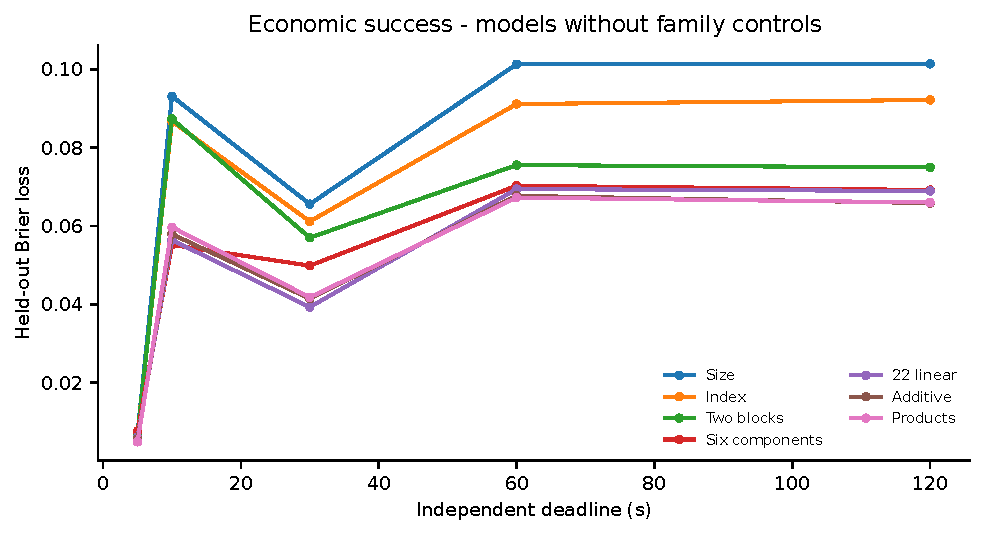
\includegraphics[width=.94\linewidth]{paper1/results/prediction_economic_5_family0.pdf}
\caption{Economic-endpoint Brier loss without family controls. Curves connect independent deadline-specific fits; they are not solver trajectories.}
\label{fig:descriptions}
\end{figure}
\begin{figure}[htbp]\centering
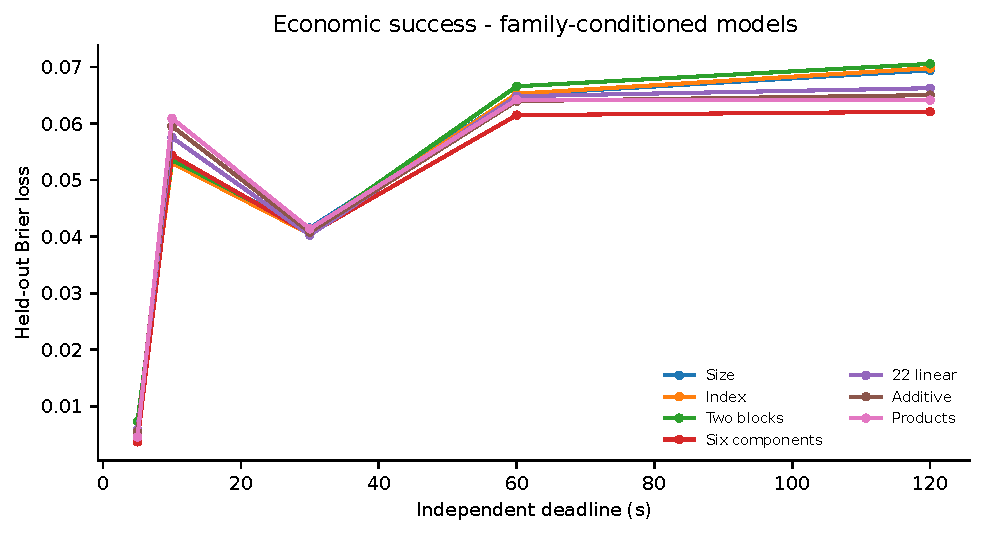
\includegraphics[width=.94\linewidth]{paper1/results/prediction_economic_5_family1.pdf}
\caption{Economic-endpoint Brier loss conditional on the known sampling regime. This tests residual refinement after family information is supplied, not the scalar's total predictive value. The six-component description improves the 120-second result. The vertical scale differs from Figure~\ref{fig:descriptions}.}
\label{fig:descriptions_family}
\end{figure}

\subsection{Discrimination and calibration}
At 120 seconds, the family-adjusted six-component model achieves ROC
areas of 0.9558 for E and 0.9580 for ES. These discrimination scores do
not by themselves validate its probabilities. In the highest probability
bin, E has 421 scenarios with mean prediction 0.9893 and observed success
0.9857; ES has 399 scenarios with corresponding values 0.9867 and 0.9875.
The other bins contain only 10--34 scenarios for E and 13--47 for ES,
with wide intervals and some material local discrepancies. For example,
the E bin with mean prediction 0.5579 has observed success 0.3000
on ten scenarios, with interval [0, 0.6000].
Calibration is therefore more precisely characterized near the abundant
high-probability outcomes than in the intermediate range; a routing risk
guarantee is not established by these development plots.

\subsection{Do changing scales explain deadline-specific weights?}

\label{sec:revision_scale}

The intermediate model preserves one nonnegative normalized direction while allowing a separate nonnegative amplitude and intercept at each deadline. It is fitted with three fixed initializations and a ridge penalty on the effective coefficients; all tuning remains inside the training folds. The separate model selects its penalty separately for each deadline.

The common-direction model reduces pooled MSE by 11.9--40.0\% relative to the common-coefficient fit. Allowing the direction also to change reduces MSE by another 24.3--36.1\% (Table~\ref{tab:revision_models}). Thus amplitude changes explain a substantial, preference-dependent part of the original gain, but do not account for it completely.

Of the 25 preference--deadline contrasts between the common-direction and separate models, 23 have positive lower bounds in the joint scenario-bootstrap simultaneous intervals over all 50 primary contrasts. These approximate intervals condition on the held-out predictions and do not include model-refitting uncertainty. A nonsignificant contrast is not evidence of equivalence; the declared exploratory margin is 0.001 absolute MSE.

\begin{table}[htbp]\centering\small\begin{tabular}{lrrrrrr}\toprule

Preference & Common & Scaled & Separate & B1 & B1+B3+B4 & Boosting\\\midrule

Equal & 0.02767 & 0.02000 & 0.01353 & 0.02245 & 0.01801 & 0.00962\\

Cost & 0.03985 & 0.03443 & 0.02371 & 0.03926 & 0.03015 & 0.01483\\

Direct thermal CO$_2$ & 0.03855 & 0.02315 & 0.01753 & 0.02397 & 0.02156 & 0.01275\\

Time & 0.01550 & 0.01366 & 0.00873 & 0.01838 & 0.01347 & 0.00682\\

Service & 0.03739 & 0.02385 & 0.01728 & 0.02546 & 0.02205 & 0.01260\\

\bottomrule\end{tabular}\caption{Nested held-out MSE over 3,000 observations per preference. Scaled denotes the common-direction model. B1 and the compact model have deadline-specific coefficients, as does boosting. These comparisons use the original five scenario folds of the weight study.}\label{tab:revision_models}\end{table}

\begin{figure}[htbp]\centering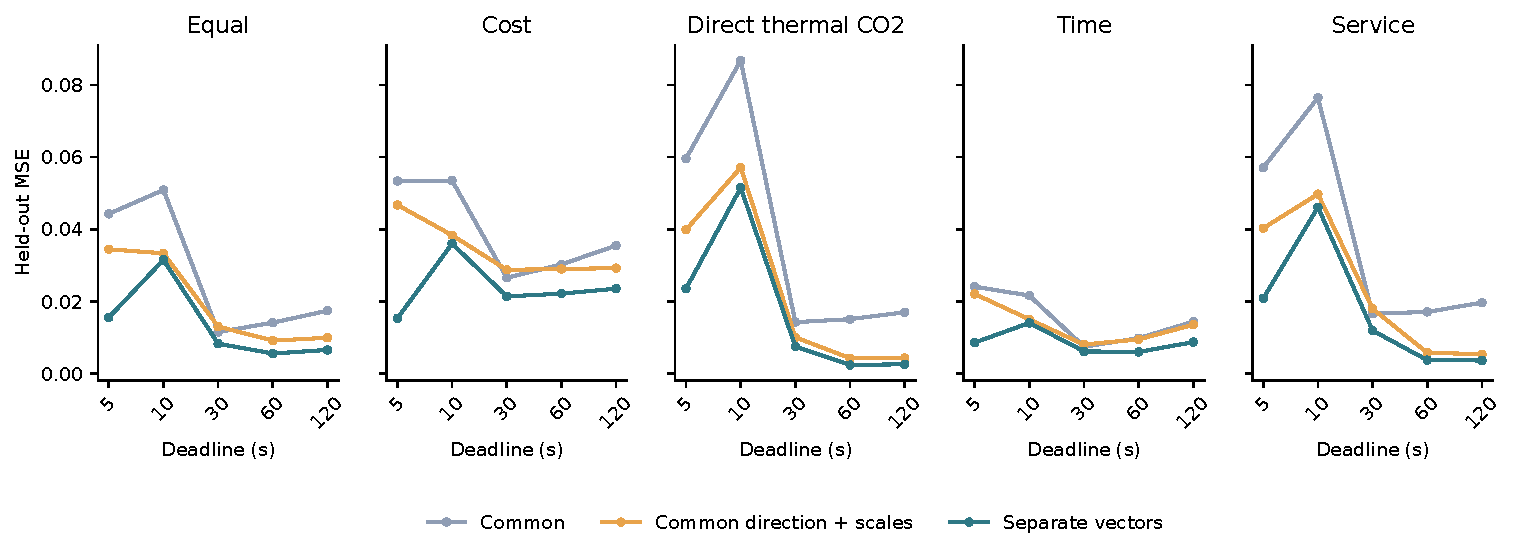
\includegraphics[width=\linewidth]{paper1/results/revision_scale_direction.pdf}\caption{Separating amplitude and direction changes using independent deadline-specific observations.}\end{figure}

\subsection{How much representation is necessary?}

\label{sec:revision_compact}

The 22-component separate model improves on B1 alone and on B1+B3+B4 for each pooled preference, but the flexible boosting model is more accurate for all five. The linear index is therefore an interpretability--accuracy compromise. Removing training-fold constants and correlations above 0.95 produces nearly unchanged losses; this is evidence against treating all 22 entries as distinct empirically identified dimensions. Fixed grouping of (A2,A4), (A3,A5) and (A7,A8), and a separate nonsaturating transformation of A6 and B8 are reported in the reproducibility tables. These are evaluated alternative representations, not silent changes to the historical index.

\subsection{What is predicted: delivery, quality or service?}

\label{sec:revision_failures}

At 5 seconds, 468 of 600 runs do not deliver a valid dispatch on time, 28 deliver but fail economic quality, and 3 pass economics but fail service. At 120 seconds, all deliver, 95 fail economics and 30 additional runs fail service. This decomposition separates pipeline delivery difficulty from the quality of a delivered dispatch (Figure~\ref{fig:revision_failures}).

\begin{figure}[htbp]\centering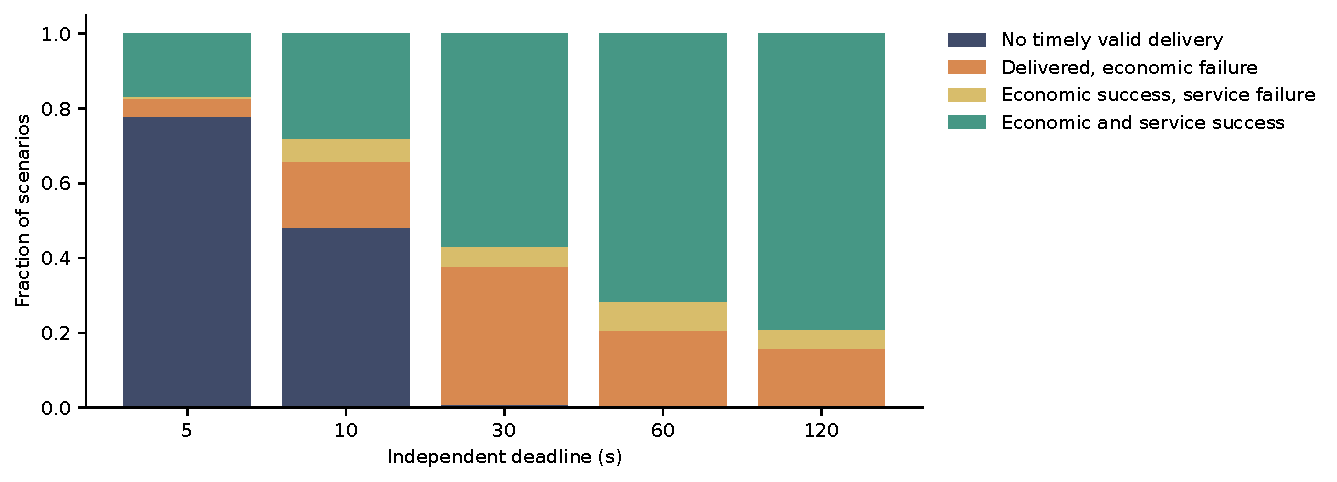
\includegraphics[width=.94\linewidth]{paper1/results/revision_failure_decomposition.pdf}\caption{Mutually exclusive observed outcomes. Short deadlines predominantly assess delivery of the complete computational pipeline.}\label{fig:revision_failures}\end{figure}

Conditional fractional-logistic fits estimate delivery, economic success given delivery, and service given economic success. Shared tuning of the conditional factors guarantees $\widehat P(ES)\leq\widehat P(E)$. A continuous two-part model combines non-delivery probability with the conditional bounded loss. Projection of linear predictions onto $[0,1]$ is also reported; it cannot increase squared error for this target. Calibration bins and their counts are included in the supplement.

\subsection{How far do the findings transfer?}

\label{sec:revision_transfer}

Leaving one complete family out, with leave-one-family-out tuning among the remaining five, reveals substantial deterioration. Family labels are excluded from all predictors. This assesses transfer among the six constructed regimes, not an independent external system.

\begin{table}[htbp]\centering\small\begin{tabular}{lrrr}\toprule Preference & Within-family folds & Held-out family & Ratio\\\midrule

Equal & 0.01353 & 0.04310 & 3.19\\

Cost & 0.02371 & 0.08601 & 3.63\\

Direct thermal CO$_2$ & 0.01753 & 0.04771 & 2.72\\

Time & 0.00873 & 0.03158 & 3.62\\

Service & 0.01728 & 0.05152 & 2.98\\

\bottomrule\end{tabular}\caption{Pooled MSE of separate 22-component models under the two validation designs. Ratios describe the change of evaluation distribution; they are not paired causal effects.}\label{tab:revision_transfer}\end{table}

The independent physical campaign is in progress: four batches of 100 fresh scenarios cover unfiltered draws, temporal structure, topology and decoupled parameters. Its predictors were frozen before execution and remain unchanged. No independent performance estimate is reported here (Section~\ref{sec:evidence_status}). Horizon coefficients remain unidentified in the historical training population.

\subsection{Can the descriptors improve a time-allocation decision?}

\label{sec:revision_allocation}

Within each outer test fold, an exact multiple-choice budget allocation maximizes predicted ES success subject to a sum of reserved deadlines. The model has seen none of the scenarios in that portfolio. E is a secondary endpoint. Uniform allocations, a predetermined adjacent-deadline mixture, size-only predictions, the original index, B1+B3+B4 and the observed-outcome oracle use the same budget constraint.

\begin{table}[htbp]\centering\small\begin{tabular}{rrrrrrr}\toprule Mean seconds & Uniform & Size & Index & Compact & 22 & Oracle\\\midrule

10 & 168 & 231 & 218 & 256 & 249 & 273\\

20 & 265 & 344 & 322 & 364 & 359 & 417\\

30 & 341 & 395 & 378 & 413 & 415 & 472\\

60 & 430 & 451 & 450 & 464 & 459 & 475\\

\bottomrule\end{tabular}\caption{Observed ES successes across five disjoint test portfolios, totaling 600 scenarios. The oracle uses observed outcomes, not true success probabilities.}\label{tab:revision_allocation}\end{table}

The compact representation matches or exceeds the 22-component allocation at three of the four budgets, despite its higher continuous prediction loss. Predictive accuracy and decision utility therefore yield different representation choices. Portfolio bootstrap intervals resample scenarios and reoptimize the allocation within each fold; models remain fixed. Reserved seconds and observed process-exit seconds are recorded separately. No observed portfolio exceeds its total reserve, but these retrospective sums do not establish a strict real-time guarantee or include the online cost of feature computation and allocation.

\begin{figure}[htbp]\centering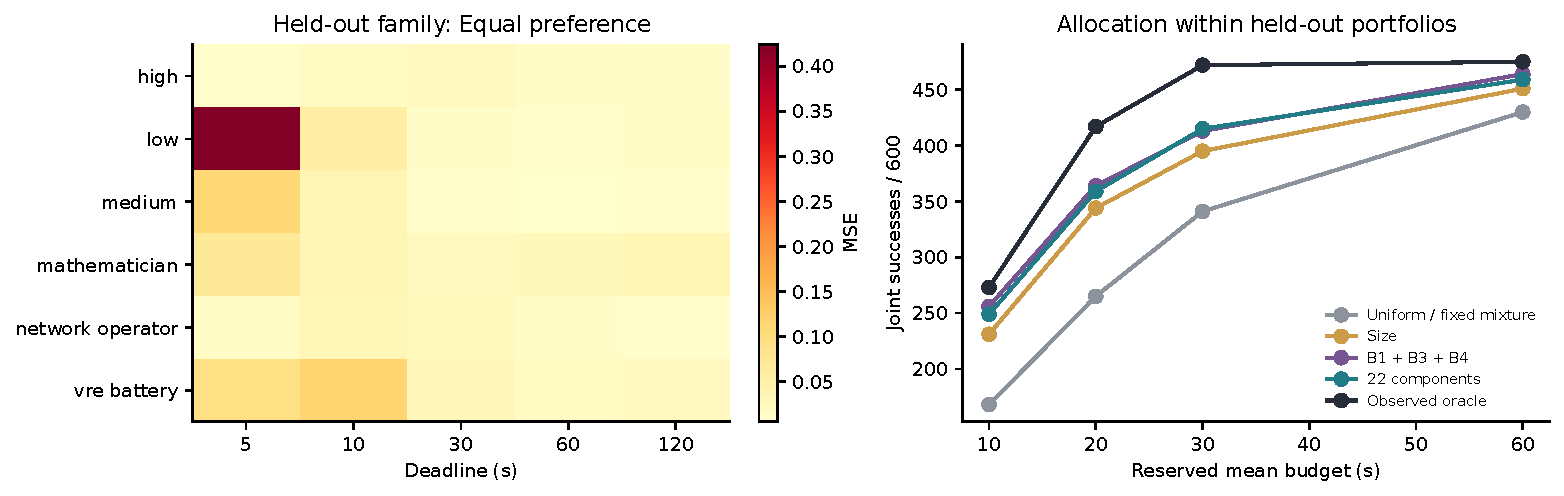
\includegraphics[width=\linewidth]{paper1/results/revision_transfer_allocation.pdf}\caption{Family transfer for the equal preference (left) and retrospective ES budget allocation (right). Predictive generalization is limited while within-regime decision utility can remain useful.}\end{figure}

\subsection{Realized descriptors: extrapolation and bounded alternatives}
\label{sec:bounded_results}
The historical follow-up in Section~\ref{sec:bounded_method} first reveals a
specific extrapolation failure. All historical networks are trees, so
$B9^{\rm M}=|\mathcal L|/N=1-1/N$. When the low-criticality family is excluded,
training cases contain 30--170 zones, compared with 4--30 in the omitted
family. The training mean and standard deviation of $B9^{\rm M}$ are
0.98940 and 0.00443. A four-zone case has $B9^{\rm M}=0.75$, or approximately
$-54.0$ training standard deviations. For the service preference at five
seconds, its B9 contribution is $-7.08793$, yielding an affine prediction
of $-5.94420$ against an observed target of 0.04046. Positive coefficients
do not prevent a negative prediction when centered features extrapolate.

Across 100 omitted low-criticality scenarios, five deadlines and five
preferences, 2,216 of 2,500 realized-descriptor linear predictions are
negative. B9 supplies the most negative additive contribution in 1,898 of
these cases. These are repeated predictions on 100 scenarios, not 2,500
independent instances. The explanation is an exact decomposition of the
fitted predictor, not evidence that B9 physically causes solver difficulty.

Projecting both representations' saved linear predictions onto $[0,1]$
reverses the aggregate comparison: realized descriptors reduce family-held-out
MSE by 18.6--51.3\% relative to projected generator descriptors, depending on
preference. Thus the very large unprojected losses should not be interpreted
as a general failure of the realized feature set. Projection nevertheless
collapses many easy-case predictions to zero and leaves other transfer errors.

\begin{table}[htbp]\centering\small
\begin{tabular}{lrrrr}\toprule
Preference & \shortstack{Projected\\linear} & \shortstack{Linear\\without B9} & \shortstack{Fractional\\logit} & \shortstack{Fractional logit\\without B9}\\\midrule
\multicolumn{5}{l}{\textit{Scenario-grouped validation}}\\
Equal & 0.01337 & 0.01401 & 0.00992 & 0.00992\\
Cost & 0.02313 & 0.02386 & 0.01605 & 0.01604\\
CO$_2$ & 0.01705 & 0.01748 & 0.01317 & 0.01317\\
Time & 0.00828 & 0.00899 & 0.00660 & 0.00670\\
Service & 0.01694 & 0.01757 & 0.01253 & 0.01253\\
\addlinespace
\multicolumn{5}{l}{\textit{Family-held-out validation}}\\
Equal & 0.03605 & 0.05384 & 0.01504 & 0.01451\\
Cost & 0.06047 & 0.08298 & 0.02529 & 0.02491\\
CO$_2$ & 0.03376 & 0.05674 & 0.02437 & 0.01943\\
Time & 0.01774 & 0.03702 & 0.01314 & 0.01099\\
Service & 0.04410 & 0.06225 & 0.01776 & 0.01730\\
\bottomrule
\end{tabular}
\caption{Exploratory historical MSE using realized MILP descriptors. Each cell averages 3,000 observations (600 scenarios, five deadlines). Both linear columns deliver predictions projected onto $[0,1]$; fractional-logistic outputs are bounded by their link. Models and tuning are specific to each deadline. The independent campaign contributes no outcomes.}\label{tab:bounded_milp}
\end{table}


The fractional-logistic model with B9 removed reduces MSE relative to the
projected realized-descriptor comparator by 19.1--30.6\% under scenario folds
and by 38.1--60.8\% under family holdout (Table~\ref{tab:bounded_milp}). All
five pooled contrasts in each scheme have positive lower bounds in the
conditional simultaneous intervals. Removing B9 from the linear model alone
instead increases MSE by 2.5--8.6\% and 37.2--108.7\%, respectively. The
choice of predictive model therefore changes the interpretation of ablation:
B9 can be useful to the linear approximation even though its extrapolation
requires control.

Within the bounded model, B9 removal further improves all five family-held-out
losses, with positive conditional simultaneous lower bounds. The additional
MSE reductions range from 1.5\% to 20.3\% relative to the full bounded model.
Under scenario folds, effects are negligible for four preferences, and the
time-priority MSE increases by 1.5\%. The historical transfer evidence favors
the bounded model without B9 as a candidate, without establishing a universal
advantage for dropping that coordinate.

The original generator descriptors also benefit from fractional-logistic
fitting (Appendix~\ref{app:bounded_followup}). With the same bounded model
and B9 ablation, realized descriptors have lower MSE for all five preferences
under scenario folds and for four under family holdout. The exception is
CO$_2$ priority, whose family-held-out MSE is 2.7\% higher. Accordingly, the
large improvements over projected linear predictions must not be attributed
entirely to descriptor recomputation.

Transfer remains imperfect. For the bounded realized model without B9,
family-held-out MSE is 1.38--1.64 times the corresponding scenario-fold MSE.
Within the low-criticality family itself, four preferences improve relative
to the projected comparator, but time-priority MSE rises from 0.01006 to
0.01293. These historical results neither establish deployment calibration
nor revise the ES-allocation results in Section~\ref{sec:revision_allocation}.
No outcome from the independent campaign is used in these fits or comparisons.


\section{Discussion}
\subsection{Criticality is informative, but its aggregation is consequential}
The reference indicator contains predictive information about timely
operational success beyond the observed size dimension. The pooled scalar
improves Brier loss in seven of ten endpoint--deadline comparisons, while
separate component descriptions can improve prediction further. This
supports criticality as an interpretable description of the sampled energy
systems. It also shows the cost of compressing distinct physical and
structural dimensions into one fixed scalar.

Arithmetic sensitivity and predictive information remain separate. B8 and
B4 have the strongest effects on scenario order under component removal,
whereas short-deadline predictive contrasts highlight demand-response
headroom A10 and ramp tightness B7, and B3 contributes at 30 seconds. Only
six of 80 pooled component-removal Brier intervals have positive lower bounds.
No component ordering is established across all deadlines, and the five
targeted products do not consistently outperform flexible additive
associations. The evidence favors retaining the decomposition rather than
interpreting the largest arithmetic contribution as the dominant mechanism.

\subsection{What preference-dependent weights measure}
\label{sec:p1_index_construction}
The five regressions ask how normalized descriptors should be combined to
anticipate a declared continuous operational loss. The coefficients
$\pi^{(p)}$ define priorities among outcomes; learned weights $w^{(p)}$
describe associations between scenario components and that target. The two
sets of weights must be distinguished. A high weight on renewable
penetration under a carbon-oriented preference can reflect the probability
of non-delivery rather than thermal emissions conditional on delivery.

Deadline dependence has an operational interpretation. At five seconds,
the common failure penalty dominates many targets, so learning primarily
separates scenarios for which dispatch delivery is possible. At longer
deadlines, almost every scenario receives a valid dispatch; remaining
differences concern economic quality, service, thermal generation and
completion time. Changes in leading weights are consistent with this
changing composition of the response. They do not establish that physical
causes of difficulty change in the same proportions.

All five common nonnegative fits improve on the recalibrated reference
indicator. Separate deadline-specific vectors yield an additional
40.5--54.5\% reduction in held-out MSE. This supports conditioning predictive
models on available time and operational preference. However, separate
models change both normalized weights and total coefficient scale. The
intermediate model with shared weights and deadline-specific
slopes explains part, but not all, of the gain: the remaining pooled
reduction is 24.3--36.1\%, with 23 of 25 deadline-specific contrasts positive
under the simultaneous analysis. These results identify conditional
candidate indicators rather than proving that every common weighting is
inadequate.

Nonnegativity preserves the intended direction of a severity indicator,
but is a modeling assumption. The historical affine models can exceed the
target's $[0,1]$ range. The separate fractional-logistic follow-up enforces
the range and improves historical predictive loss, but boundedness alone
does not establish calibration or deployment validity. Its coefficients
act on a transformed conditional mean and do not redefine the original
additive indicator. Additive preferences also allow compensation between criteria.
A low composite loss does not guarantee continuity of service; a mandatory
ENS cap must remain an explicit condition when required operationally.
The carbon criterion concerns direct internal thermal emissions per served
MWh and cannot establish a consumption footprint or carbon-optimal dispatch.

\subsection{Redundancy, sampling design and limits of generalization}
Pearson correlations are 0.99998 between A3 and A5, 0.97633 between A7 and
A8, and 0.92205 between A2 and A4. Equal weights can give repeated influence
to a shared dimension, while fitted coefficients can exchange weight between
nearly equivalent descriptions. These associations concern the sampled
support rather than universal equivalence. Training-fold redundancy reduction now yields nearly unchanged predictive
loss, while fixed grouping has small costs. The historical definition remains
the common reference; alternative representations are explicitly versioned.

Constant and saturated components introduce further limits. B2 contains
no horizon variation and B5 is a constant proxy. Their weights cannot be
identified here; zero coefficients do not justify general exclusion.
Clipping of A6 in 63.8\% and B8 in 33.8\% of scenarios removes information
about extremes. Fixed normalization enables consistent comparisons but may
lose discrimination under shifted conditions. Revising proxy definitions
or bounds would define a new indicator requiring evaluation.

Family-conditioned models address refinement after the sampling regime is
known. Because families use targeted parameter spaces and criticality-based
selection, small residual scalar gains do not contradict pooled findings.
Conversely, pooled predictive value does not demonstrate transfer to
independently sampled systems. At 120 seconds, the six-component
family-conditioned Brier gains of 0.00732 for E and 0.00851 for ES are
concentrated mainly in the mathematician family. A benefit in that regime
cannot be assumed to hold across all structures.

Nested scenario-grouped validation prevents related observations from
crossing training and validation boundaries. It does not remove the
exploratory character of a previously inspected cohort or substitute for
external validation. Loss intervals condition on out-of-fold predictions;
weight intervals refit coefficients while holding the selected ridge
penalty fixed. Neither accounts for all model-selection uncertainty, and
the historical pointwise intervals do not correct for the many comparisons.
The revision adds joint simultaneous intervals for its 50 declared primary
scale/direction contrasts, while secondary sensitivities remain exploratory. Small isolated
gains and component rankings remain hypotheses for confirmation. New
horizons, independently varying networks, alternative sampling distributions
and other solvers are needed to assess transportability.

The realized-descriptor follow-up further separates feature semantics from
the predictive model. On the historical trees, $B9^{\rm M}=1-1/N$ is a size
transformation rather than an independently varying topology descriptor.
Its small training variance can amplify affine extrapolation. Nevertheless,
removing it alone worsens the projected linear predictor; the improvement
from removal depends on using the bounded model. The joint change of link
and fitting loss also helps the original generator descriptors, so the full
gain cannot be credited to physical feature recomputation. Remaining
family-specific failures and the unknown cost of an online decision rule
limit the interpretation. The bounded follow-up and its simultaneous
intervals are explicitly post-hoc historical evidence, distinct from the
unchanged independent-test freeze (Section~\ref{sec:evidence_status}).

\subsection{From scenario criticality to method complementarity}
The present study characterizes difficulty encountered by direct HiGHS
optimization. Predicting that a scenario is difficult for this method does
not identify which alternative can satisfy the same request. An alternative
may preserve service more reliably but incur higher cost, or produce an
acceptable result earlier without improving economic quality. These
differences require method-specific observations under the same physical
model, validity checks and complete-execution deadlines.

Subsequent work could extend the analysis from scenario criticality to
the operational service delivered by each method, comparing
direct optimization, rolling-horizon construction, a learned single-candidate
method and an energy-guided candidate portfolio. The criticality components
provide a vocabulary for examining where their time--cost--service trade-offs
differ. Variability, storage adequacy and state-of-charge restrictions, for
example, motivate hypotheses about renewable/battery scenarios, while
combinatorial and ramping descriptors motivate comparisons in structurally
constrained systems. These hypotheses must be tested against method outcomes;
the present coefficients do not establish their mechanisms.

This distinction clarifies the progression toward algorithm selection
\citep{rice1976,bischl2016}. This paper establishes whether scenario
descriptions contain predictive information. Subsequent work would need to
establish whether methods offer complementary operational outcomes. Only when complementarity
exists can a subsequent selection rule seek to improve on a fixed method,
accounting for feature computation and selection time. This separates
predictive evidence from cross-method selection. Within-method budget
allocation has now been evaluated in Section~\ref{sec:revision_allocation};
it does not identify which alternative optimization method to choose.

\section{Conclusion}
Scenario criticality contains useful information about timely economic and
service outcomes within the six sampled regimes. The numerical indicator
must nevertheless be distinguished from the underlying deterministic
scenario and its realized MILP. In particular, the audited A3 proxy repeats
demand-scale information and does not measure a realized peak-to-valley ratio.

Deadline-specific rescaling explains part of the improvement previously
attributed jointly to scale and weights. Separate weight directions still
reduce pooled MSE by 24.3--36.1\% beyond this intermediate model, but
nonlinear predictions are more accurate and redundant components can be
removed with little loss. For that original normalized linear comparator,
leaving a complete family out multiplies MSE by 2.72--3.63, materially
restricting transportability claims.

An exploratory follow-up on realized MILP descriptors diagnoses large
negative affine extrapolations of the line-to-zone coordinate. Positive
fractional-logistic regression without B9 reduces MSE by 19.1--30.6\%
under scenario folds and 38.1--60.8\% under family holdout relative to the
projected realized-descriptor linear comparator. B9 removal alone instead
degrades that linear predictor. The original generator descriptors also
benefit from bounded regression, and some family-specific errors remain.
These findings motivate a bounded predictive candidate, not a universally
validated criticality index or a new operational allocation result.

Retrospective allocation within held-out portfolios establishes a limited
decision use: 415 joint successes versus 341 under uniform allocation at a
30-second average reserve. A compact structural representation performs
similarly, so the most accurate continuous predictor is not automatically
the best choice for this decision. These findings remain conditional on
historical observations, HiGHS and the declared preferences. The independent
400-scenario campaign, stronger references and instrumented repetitions
are in progress. Their pre-execution frozen predictors remain unchanged;
the post-hoc bounded models are separate. No independent performance result
is used to support the present conclusions.

\appendix
\section{Operational MILP and scenario-to-model mapping}
\label{app:milp}
This appendix describes the implemented formulation, not a generic unit
commitment model. All parameters below are fixed by scenario $s$.
The code-level specification is \texttt{src/milp/model.py}, with the
time-unit correction and independent validator in
\texttt{src/operational\_exit/physics.py}. The reproducibility archive
records their exact hashes and the scenario loader and profile generator.

\paragraph{Indices, variables and aggregation.}
Let $z\in\mathcal Z$, $t=1,\ldots,T$, $\ell\in\mathcal L$ and
$k\in\mathcal K_{\rm DR}$ index zones, time, transport lines and response
cost blocks. Powers and flows are in MW; stored and deferred energy are in
MWh; $\Delta t$ is in hours. Continuous nonnegative variables are thermal,
nuclear, solar, wind and hydro generation $p^{\rm th},p^{\rm nu},p^{\rm sol},
p^{\rm wind},h$; renewable and hydro spill; battery and pumped charge,
discharge and energy; deferred power $d$, recovered power $r$, backlog $q$;
ENS $e$; overgeneration spill $o$; and system imports $m^+$ and exports $m^-$.
Transport flows $f_{\ell t}$ may be positive or negative. Binary variables
are thermal on/off $u_{zt}$ and start-up $v_{zt}$, deferral activation $a_{zt}$,
battery/pumped charge modes $c^B_{zt},c^P_{zt}$ and import mode $i_t$.
There is one thermal commitment per zone and time, not one per installed
thermal unit. Nuclear output is continuous and subject to minimum output;
there is no nuclear commitment binary. Shutdown is the expression
$w_{zt}=u_{z,t-1}-u_{zt}+v_{zt}$, not an additional decision variable.

\paragraph{Generator metadata are not always active physical controls.}
The historical JSON files omit the optional unit-capacity override block.
Installed battery energy therefore equals installed battery power times the
loader's default four hours. The sampled field
\path{battery_e_to_p_hours} enters generator flexibility summaries and B8,
but does not change that installed duration in this cohort. Likewise,
\path{dr_duration_hours} does not impose a maximum deferral duration in the
implemented lossless-backlog constraints, and the nominal hydro head-efficiency
field is not an extra multiplier in the nodal balance. These legacy fields
must not be described as independently varied physical constraints. Their
predictive associations can reflect sampling correlations. New physical
duration experiments must explicitly change realized power/energy arrays,
as the prepared decoupling batch does.

\paragraph{Objective.}
The validated objective, including trade credits and unserved-energy cost, is
\begin{align}
 \min\ C={}&\sum_{z,t} c^{\rm start}_zv_{zt}
 +\Delta t\sum_{z,t}\left(c^{\rm th}_zp^{\rm th}_{zt}
 +c^{\rm nu}_zp^{\rm nu}_{zt}+\sum_k c^{\rm DR}_kd_{ztk}
 +V e_{zt}+c^{\rm ren}(s^{\rm sol}_{zt}+s^{\rm wind}_{zt})\right.\nonumber\\
 &\left.\qquad+c^{\rm hydro}s^H_{zt}+c^o o_{zt}
 +c^B_z(p^{B+}_{zt}+p^{B-}_{zt})
 +c^P_z(p^{P+}_{zt}+p^{P-}_{zt})\right)\nonumber\\
 &+\Delta t\sum_t(c^{\rm imp}m^+_t+c^{\rm exp}m^-_t).
\end{align}
Here $c^{\rm exp}$ is negative. The thermal energy cost includes fuel,
the variable operating adder and $0.72$ times the carbon price.
Start-up costs are charged per event, without multiplication by $\Delta t$.
The historical references may consequently have negative total cost.
The metadata nuclear start-up cost does not enter an additional nuclear
commitment term in this implemented MILP.

\paragraph{Thermal and nuclear operation.}
Initial output and on/off state are scenario parameters. For every zone and
time, thermal constraints are
\begin{align}
 \underline P^{\rm th}_zu_{zt}&\le p^{\rm th}_{zt}\le\overline P^{\rm th}_zu_{zt},\\
 v_{zt}&\ge u_{zt}-u_{z,t-1},\quad
 v_{zt}\le u_{zt},\quad v_{zt}\le1-u_{z,t-1},\\
 p^{\rm th}_{zt}-p^{\rm th}_{z,t-1}
 &\le R_zu_{z,t-1}+SU_zv_{zt},\\
 p^{\rm th}_{z,t-1}-p^{\rm th}_{zt}
 &\le R_zu_{zt}+SD_zw_{zt}.
\end{align}
The shared thermal-limit routine determines $SU_z,SD_z$ and initial status;
the inequalities apply also at the first step using those initial values.
No thermal minimum-up/down-duration constraints are imposed. Nuclear output
satisfies $\underline P^{\rm nu}_z\le p^{\rm nu}_{zt}\le\overline P^{\rm nu}_z$
and $|p^{\rm nu}_{zt}-p^{\rm nu}_{z,t-1}|\le0.5\overline P^{\rm nu}_z$ for
$t>1$. Solar and wind each satisfy $p^{j}_{zt}+s^{j}_{zt}=\overline P^j_{zt}$.

\paragraph{Lossless deferred demand.}
Block variables sum to total deferral:
\begin{align}
 d_{zt}&=\sum_kd_{ztk},\quad0\le d_{ztk}\le\overline D_{ztk},\quad
 0.1a_{zt}\le d_{zt}\le\overline D_{zt}a_{zt},\\
 0\le r_{zt}&\le\overline R_{zt}(1-a_{zt}),\quad
 q_{zt}=q_{z,t-1}+\Delta t(d_{zt}-r_{zt}),\\
 \Delta t\,r_{zt}&\le q_{z,t-1},\quad q_{z0}=q_{zT}=0,\quad q_{zt}\ge0,\\
 \sum_t a_{zt}&\le M_z,\qquad |d_{zt}-d_{z,t-1}|\le R^{\rm DR}_z\quad(t>1).
\end{align}
The parameter historically named \texttt{dr\_max\_events} limits active
periods, not activation starts. The legacy minimum-duration field does not
add a minimum-duration constraint. Rebound decay and terminal backlog
tolerance fields do not override the implemented lossless balance and exact
terminal repayment. Unserved energy $e$ is a separate penalized variable;
it is never identified with temporary deferral $d$.

\paragraph{Storage and hydro.}
For $j\in\{B,P\}$ (battery or pumped storage),
\begin{align}
 0\le p^{j+}_{zt}&\le\overline P^j_zc^j_{zt},\quad
 0\le p^{j-}_{zt}\le\overline P^j_z(1-c^j_{zt}),\\
 E^j_{zt}&=\rho^j_zE^j_{z,t-1}
 +\Delta t\left(\eta^{j+}p^{j+}_{zt}-p^{j-}_{zt}/\max(\eta^{j-},10^{-4})\right),\\
 0\le E^j_{zt}&\le\overline E^j_z,\qquad
 \underline E^j_{zT}\le E^j_{zT}\le\overline E^j_{zT}.
\end{align}
Initial levels are fixed. Terminal inequalities are activated in the code
when the associated capacity and bound exceed $10^{-6}$; otherwise the
ordinary nonnegativity/capacity bounds apply. Zero-energy pumped devices
have their level fixed to zero. Reservoir hydro satisfies
\begin{equation}
 H_{zt}=H_{z,t-1}+\Delta t(I_{zt}-h_{zt}-s^H_{zt}),\quad
 0\le H_{zt}\le\overline H_z,\quad0\le h_{zt}\le\overline P^H_z,
\end{equation}
with fixed initial reservoir level; no reservoir terminal target is imposed.
Zero-energy reservoirs are fixed to zero. Run-of-river generation is fixed
scenario input. Hydro release is already represented as electrical power
in the balance; no additional efficiency multiplier is inserted there.

\paragraph{Transport, trade and power balance.}
Let $A_{z\ell}$ be $+1$ at the receiving endpoint and $-1$ at the sending
endpoint, and $z_0$ the import/export anchor zone. Then
\begin{align}
 -\overline F_\ell&\le f_{\ell t}\le\overline F_\ell,\qquad
 0\le m^+_t\le\overline M i_t,\quad0\le m^-_t\le\overline M(1-i_t),\\
 &p^{\rm th}_{zt}+p^{\rm nu}_{zt}+p^{\rm sol}_{zt}+p^{\rm wind}_{zt}
 +h_{zt}+p^{\rm ror}_{zt}+p^{B-}_{zt}+p^{P-}_{zt}
 +\sum_\ell A_{z\ell}f_{\ell t}\nonumber\\
 &\quad+\ind\{z=z_0\}(m^+_t-m^-_t)+d_{zt}+e_{zt}
 =D_{zt}+r_{zt}+p^{B+}_{zt}+p^{P+}_{zt}+o_{zt}.
\end{align}
There are no electrical angles, Kirchhoff loop equations, AC losses or
security contingencies. Binary variables attached to absent thermal,
storage, response or trade capacity are fixed to zero. These structural
fixings are one reason the generator estimate B3 is not a count of actual
free binary variables.

\section{Additional revision protocols and reproducibility}
\label{app:revision_protocol}
The common-direction regression is
\begin{equation}
 \widehat Y^{(p)}_{sb}=a^{(p)}_b+\alpha^{(p)}_b\sum_jw^{(p)}_jz_{sj},
 \quad w_j\ge0,\quad\sum_jw_j=1,\quad\alpha_b\ge0.
\end{equation}
Its objective is the mean squared loss over scenarios and deadlines plus
$\lambda |\mathcal D|^{-1}\sum_b\|\alpha_bw\|_2^2$. This reduces to the
common-vector penalty when all amplitudes are equal. Alternating
nonnegative least squares uses pooled, uniform-active and B1-coordinate
initializations for the full design; other representations use their first
coordinate when B1 is absent. Initialization objectives, convergence and
outer-fold group-weight sums are retained. A shared direction is not
claimed globally optimal merely because the alternating procedure converges.

The conditional models use a fractional Bernoulli quasi-likelihood with
logistic link; binary targets are its special case. Training subsets are
restricted to the stated conditioning event. Single-class subsets use the
observed constant; empty subsets use 0.5 and other subsets with fewer than
ten observations use Laplace-smoothed frequency. A common penalty for the
E/ES factors is selected by their mean inner-fold Brier loss, preserving
probability ordering. For continuous loss,
\begin{equation}
 \widehat{\mathbb E}[Y^{(p)}\mid x,b]
 =1-\widehat P(F\mid x,b)
 +\widehat P(F\mid x,b)\widehat{\mathbb E}[Y^{(p)}\mid F,x,b].
\end{equation}
The linear candidate grid is $\{0,10^{-4},10^{-3},10^{-2},10^{-1},1,10\}$;
constant and original-index fits remain unpenalized. Boosting uses 100
iterations, learning rate 0.05, leaf counts selected from $\{7,15,31\}$,
minimum leaf size 20 and $L_2=1$, with early stopping disabled. Reduced
features are chosen inside each training fold by discarding constants
and then correlations exceeding 0.95 in absolute value, in fixed component
order. The nonsaturating sensitivity replaces only A6 and B8 with
$0.5+\arctan((x-\ell)/(u-\ell)-0.5)/\pi$ using their raw values.

The one-at-a-time target grid varies ENS anchors over 0.005/0.01/0.02,
cost-gap anchors over 0.025/0.05/0.10, and carbon-intensity anchors over
0.36/0.72/1.44. Priority weights are 0.4/0.6/0.8 with equal sharing of the
remainder. The physical emissions factor remains 0.72. A separate
evaluation removes ENS penalties and thermal carbon charges from both
candidate and reference costs; it evaluates the same dispatches and does
not reoptimize them. Binary label counts are checked at 1/5/10\% cost
tolerances. These are sensitivity conventions, not scientifically
estimated thresholds. Imports retain unknown emissions rather than an
assumed zero footprint.

\begin{figure}[htbp]\centering
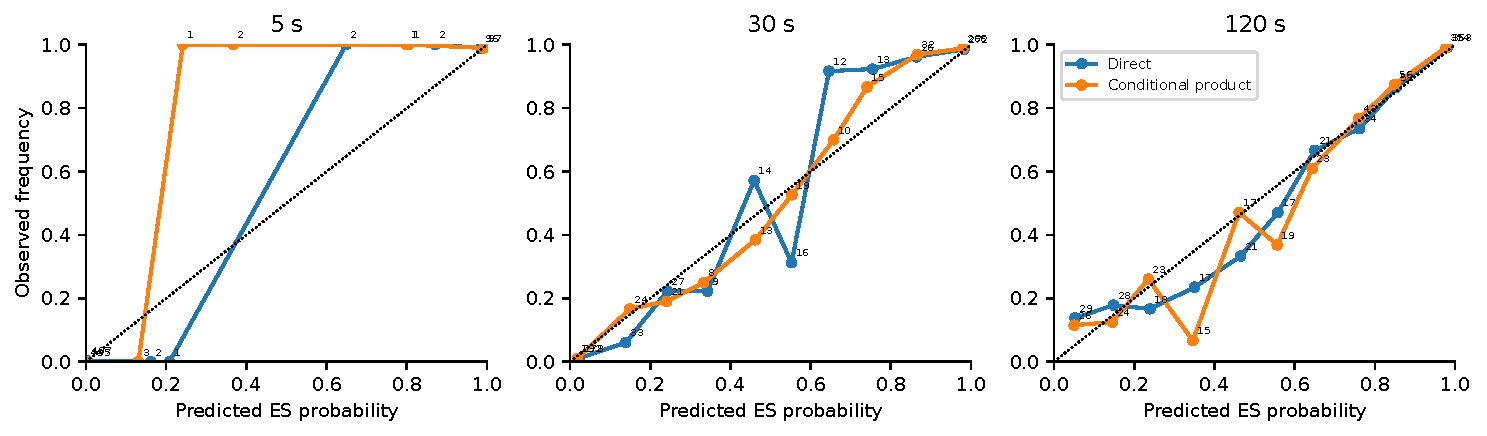
\includegraphics[width=\linewidth]{paper1/results/revision_calibration.pdf}
\caption{ES calibration in the revision models. Labels give observation
counts in fixed probability bins; sparse bins should not be overinterpreted.}
\end{figure}

The unified data contain four Parquet tables (scenarios, runs, references
and analysis) and \path{splits.json} in the isolated revision run.

All raw and normalized
descriptors, identities, families, actual available dimensions, missing
fields, reference certification and process-exit outcomes are retained.
The dictionary specifies formulas, units, input sources, floors, clipping
and fixed normalization bounds for all 22 components. Per-scenario
parameters and family-wise ranges are exported separately; the original
generator configuration and family-building scripts specify the sampling
and selection process. Historical environment versions are HiGHS 1.14.0,
Pyomo 6.10.0 and Python 3.11.9 on Windows, with 16 solver threads. Model
fitting uses the recorded numerical-library versions and one numerical
thread. Historical fold seed is 20261111; revision randomization seed is
20261112. Exact folds and per-execution seeds take precedence over a single
global seed. Historical archives do not identify all stage times or a
complete contemporaneous hardware record; these are not inferred from
total execution time or from the current machine.

The four independent batches currently being executed contain 100 cases each. Temporal
conditions are (12,60), (48,60), (72,60), (24,30), (24,120), in hours and
minutes per step. Topologies vary edges independently of zone count while
remaining connected transport networks. Decoupled conditions vary storage
power and energy factors independently over $[0.5,2]$ and reshape demand
while preserving its total energy. Both generator-proxy and realized-descriptor
predictors were frozen before the first independent attempt. Their ability
to represent the changed inputs is part of the evaluation; historically
constant coordinates still have no learned effect. The later bounded-model
follow-up is stored separately and does not replace this freeze. The strengthened
reference budget is 1,800 solver seconds with a 2,100-second process cap.
No independent performance estimate is reported in this revision. The ongoing
instrumented worker records scenario processing, model construction,
solver transfer, solution search, extraction, validation and delivery,
while the parent supervisor measures complete process exit. Partial stage
logs from interrupted runs cannot turn those runs into successes.

\section{Secondary sensitivities and execution variability}

\label{app:robustness_results}

All 48 declared preference/target specifications were fitted with the same outer folds. Across their anchor, priority and disjoint-cost variants, the pooled gain from a common direction to separate directions remains positive. This does not imply that individual coefficients or ranks are stable.

\begin{table}[htbp]\centering\small\begin{tabular}{lrr}\toprule Preference & Minimum gain (\%) & Maximum gain (\%)\\\midrule

Direct thermal CO$_2$ & 20.3 & 28.8\\

Cost & 22.4 & 32.9\\

Equal & 27.3 & 33.0\\

Service & 25.3 & 30.3\\

Time & 33.1 & 36.5\\

\bottomrule\end{tabular}\caption{Descriptive sensitivity of the pooled MSE gain from changing direction beyond deadline-specific scaling. No variant is selected using test performance.}\end{table}

\begin{table}[htbp]\centering\small\begin{tabular}{lrrr}\toprule Preference & Linear & Projected & Two-part\\\midrule

Direct thermal CO$_2$ & 0.01753 & 0.01680 & 0.01355\\

Cost & 0.02371 & 0.02208 & 0.01587\\

Equal & 0.01353 & 0.01283 & 0.01004\\

Service & 0.01728 & 0.01639 & 0.01300\\

Time & 0.00873 & 0.00823 & 0.00679\\

\bottomrule\end{tabular}\caption{Pooled held-out MSE for the separate linear, projected linear and bounded two-part models using all 22 descriptors.}\end{table}

\begin{table}[htbp]\centering\small\begin{tabular}{rrrr}\toprule Deadline (s) & Repeated cases & Variable delivery & Variable ES\\\midrule

5 & 30 & 0 & 0\\

10 & 30 & 1 & 2\\

30 & 30 & 1 & 2\\

60 & 30 & 0 & 6\\

120 & 30 & 0 & 6\\

\bottomrule\end{tabular}\caption{Cases with differing outcomes across the primary run and two archived repetitions. The 30 selected cases do not establish deployment reliability.}\end{table}

Archived logs separate aggregate computation, finalization, preload and process exit, but do not identify model construction and solver search individually. Therefore the fraction of short-deadline failures caused specifically by model construction cannot be estimated from these logs.

The 383 certified and 217 uncertified reference cases differ in family and size. Subgroup losses and case-mix tables are released without treating the certified group as representative. No numerical dual bounds were retained in the 600 archived reference records. Stronger references are being computed in the separate campaign; the complete sensitivity analysis is pending. All historical predictive results reported here retain the original reference costs and labels.

For the ES allocation, the 22-component gain over uniform allocation at 30 seconds per scenario is 74 successes; the conditional portfolio-bootstrap 95\% interval is approximately [59,90]. Relative to the size-only allocation, the point gain is 20 with interval approximately [10,31]. At 60 seconds, the gain over size is only 8 and its interval includes zero. These pointwise intervals condition on predictive fits and do not provide a simultaneous guarantee across budgets.

The full code, normalized and raw descriptors, complete held-out predictions, selected penalties, convergence diagnostics, grouped weights, scenario parameters and decision allocations are retained under \path{research/paper1_revision}. The reproduction check covers 480 historical MSE cells and 400 Brier cells, and refitted baseline predictions agree with their archived counterparts.

\section{Bounded-regression follow-up: controls and provenance}
\label{app:bounded_followup}
This supplement concerns only the historical follow-up in
Section~\ref{sec:bounded_method}. It does not report the independent campaign.
The original raw descriptors and the realized descriptors have different
semantics; applying the same model family to each helps distinguish predictive
procedure improvements from representation improvements. B9 removal refers
to the respective coordinate and does not assert that their definitions match.

\begin{table}[htbp]\centering\small
\begin{tabular}{lrrrr}\toprule
Preference & \shortstack{Projected\\linear} & \shortstack{Linear\\without B9} & \shortstack{Fractional\\logit} & \shortstack{Fractional logit\\without B9}\\\midrule
\multicolumn{5}{l}{\textit{Scenario-grouped validation}}\\
Equal & 0.01308 & 0.01324 & 0.01052 & 0.01048\\
Cost & 0.02233 & 0.02244 & 0.01631 & 0.01632\\
CO$_2$ & 0.01696 & 0.01713 & 0.01377 & 0.01372\\
Time & 0.00878 & 0.00894 & 0.00754 & 0.00752\\
Service & 0.01656 & 0.01675 & 0.01309 & 0.01302\\
\addlinespace
\multicolumn{5}{l}{\textit{Family-held-out validation}}\\
Equal & 0.04702 & 0.03996 & 0.01961 & 0.01776\\
Cost & 0.08083 & 0.07736 & 0.02957 & 0.02677\\
CO$_2$ & 0.05299 & 0.04146 & 0.01945 & 0.01891\\
Time & 0.03643 & 0.03317 & 0.02372 & 0.02149\\
Service & 0.05420 & 0.04776 & 0.02022 & 0.01866\\
\bottomrule
\end{tabular}
\caption{Exploratory historical MSE using original raw generator descriptors. Each cell averages 3,000 observations (600 scenarios, five deadlines). Both linear columns deliver predictions projected onto $[0,1]$; fractional-logistic outputs are bounded by their link. Models and tuning are specific to each deadline. The independent campaign contributes no outcomes.}\label{tab:bounded_legacy}
\end{table}

\begin{table}[htbp]\centering\small
\begin{tabular}{lrrrr}\toprule
Preference & \shortstack{Projected\\linear} & \shortstack{Linear\\without B9} & \shortstack{Fractional\\logit} & \shortstack{Fractional logit\\without B9}\\\midrule
\multicolumn{5}{l}{\textit{Low-criticality family omitted from training}}\\
Equal & 0.00560 & 0.13076 & 0.00394 & 0.00291\\
Cost & 0.01157 & 0.15537 & 0.00110 & 0.00093\\
CO$_2$ & 0.00462 & 0.13268 & 0.00360 & 0.00346\\
Time & 0.01006 & 0.10080 & 0.01602 & 0.01293\\
Service & 0.00205 & 0.14245 & 0.00116 & 0.00107\\
\bottomrule
\end{tabular}
\caption{Historical MSE on the 100 low-criticality scenarios, averaging five deadlines per scenario. The bounded model without B9 improves four preferences relative to the projected linear comparator, but time priority remains worse. These 500 rows per preference are not independent scenarios.}\label{tab:bounded_low_family}
\end{table}

\begin{table}[htbp]\centering\small
\begin{tabular}{lrrr}\toprule
Preference & MSE reduction & Lower & Upper\\\midrule
\multicolumn{4}{l}{\textit{Against projected linear: scenario folds}}\\
Equal & 0.003446 & 0.002503 & 0.004390\\
Cost & 0.007083 & 0.005680 & 0.008485\\
CO$_2$ & 0.003886 & 0.002604 & 0.005168\\
Time & 0.001578 & 0.001044 & 0.002113\\
Service & 0.004415 & 0.003163 & 0.005667\\
\addlinespace
\multicolumn{4}{l}{\textit{Against projected linear: family holdout}}\\
Equal & 0.021533 & 0.018697 & 0.024370\\
Cost & 0.035560 & 0.031872 & 0.039249\\
CO$_2$ & 0.014327 & 0.010906 & 0.017749\\
Time & 0.006752 & 0.004630 & 0.008875\\
Service & 0.026798 & 0.023384 & 0.030212\\
\addlinespace
\multicolumn{4}{l}{\textit{Against full fractional logit: family holdout}}\\
Equal & 0.000529 & 0.000357 & 0.000701\\
Cost & 0.000388 & 0.000095 & 0.000681\\
CO$_2$ & 0.004940 & 0.003519 & 0.006361\\
Time & 0.002151 & 0.001402 & 0.002900\\
Service & 0.000459 & 0.000276 & 0.000642\\
\addlinespace
\bottomrule
\end{tabular}
\caption{Positive differences favor the realized fractional-logistic model without B9. Approximate 95\% simultaneous intervals cover 40 declared contrasts within each validation scheme, with 2,000 paired scenario resamples after averaging deadlines. They condition on the fitted predictions and do not account for post-hoc design selection or refitting uncertainty.}\label{tab:bounded_contrasts}
\end{table}


The realized feature dictionary, extraction times and original frozen
comparison are retained in
\path{research/paper1_revision/runs/revision_v1/realized_milp_v1}.
The follow-up uses a separate code package,
\path{research/paper1_revision/bounded_ablation}, and separate outputs,
\path{research/paper1_revision/runs/revision_v1/bounded_ablation_v1}.
The latter contain the declared follow-up design, all 330 checkpoints,
240,000 held-out predictions including the projected comparators, losses by
family and deadline, and all 80 conditional contrasts across the two schemes.
Its declaration follows examination of historical extrapolations; it is not
a replacement for the pre-execution independent-test freeze.

Eight numerical and leakage checks passed. Replaying all 1,650 saved models
reproduced their predictions exactly, and their scaling statistics matched
their respective training folds. Delivered predictions all lie in $[0,1]$;
nonnegative slopes and optimizer stationarity were checked. No new MILP was
solved for this analysis, no independent outcome was used, and verification
of the original frozen models, predictions and source hashes was unchanged.
The manuscript tables are exported directly from the saved CSV reports;
\path{paper1/results/bounded_manuscript_provenance.json} records their sources
and hashes.

\section{Historical component and interaction ablations}
\subsection{Component contributions without family conditioning}
\label{sec:p1_components_nofamily}
The pooled removal contrasts retain the size controls and omit family
indicators. Eight components were individually tested: A2 (residual
volatility), A6 (peak-to-firm ratio), A8 (inverse storage-energy adequacy),
A10 (inverse demand-response headroom), B3 (estimated binary count),
B7 (ramp tightness), B8 (nominal SOC-tightness proxy) and B9 (regional connectivity).
These are targeted comparisons, not a predictive ranking of all 22 terms.
For each component, the full model contains all component main effects,
their fixed nonlinear basis and the five products; the reduced model
removes that component's entire block and is retuned within the same
nested folds. Define $\Delta_j=\mathrm{Brier}_{-j}-\mathrm{Brier}_{\rm full}$:
a positive value means that retaining the block improves held-out loss.
The contrast measures predictive information conditional on the other
components and size, without conditioning on the sampling-family label.

\begin{table}[htbp]\centering\small
\setlength{\tabcolsep}{4pt}
\begin{tabular}{@{}p{.10\linewidth}p{.41\linewidth}p{.41\linewidth}@{}}\toprule
Deadline (s) & E: economic success & ES: economic success and ENS\\\midrule
5 & \begin{tabular}[t]{@{}l@{}}A10: $\mathbf{1.921\ [0.013, 4.716]}$ \\
A6: $\mathbf{1.285\ [0.002, 3.131]}$ \\
B7: $0.219\ [-0.101, 0.667]$\end{tabular} & \begin{tabular}[t]{@{}l@{}}B7: $\mathbf{2.039\ [0.211, 4.607]}$ \\
A6: $1.837\ [-0.119, 4.839]$ \\
A10: $1.817\ [-0.012, 4.570]$\end{tabular} \\
\addlinespace[4pt]
10 & \begin{tabular}[t]{@{}l@{}}B3: $0.069\ [-0.352, 0.482]$\end{tabular} & \begin{tabular}[t]{@{}l@{}}A6: $0.818\ [-1.781, 3.165]$ \\
B8: $0.629\ [-2.589, 3.901]$ \\
B3: $0.285\ [-0.092, 0.668]$\end{tabular} \\
\addlinespace[4pt]
30 & \begin{tabular}[t]{@{}l@{}}B3: $\mathbf{0.536\ [0.063, 1.009]}$\end{tabular} & \begin{tabular}[t]{@{}l@{}}B3: $\mathbf{0.658\ [0.057, 1.246]}$ \\
A10: $0.464\ [-2.106, 3.024]$ \\
A8: $0.323\ [-0.102, 0.788]$\end{tabular} \\
\addlinespace[4pt]
60 & \begin{tabular}[t]{@{}l@{}}B3: $1.509\ [-0.225, 3.438]$ \\
A8: $0.474\ [-1.354, 2.518]$ \\
B8: $0.460\ [-1.535, 2.704]$\end{tabular} & \begin{tabular}[t]{@{}l@{}}A8: $0.202\ [-0.358, 0.732]$ \\
B8: $0.002\ [-0.749, 0.721]$\end{tabular} \\
\addlinespace[4pt]
120 & \begin{tabular}[t]{@{}l@{}}B9: $0.964\ [-0.870, 3.048]$ \\
B3: $0.758\ [-0.056, 1.579]$ \\
B8: $0.438\ [-0.487, 1.321]$\end{tabular} & \begin{tabular}[t]{@{}l@{}}B3: $1.231\ [-0.146, 2.553]$ \\
B8: $0.996\ [-0.985, 2.940]$ \\
B9: $0.510\ [-2.268, 3.338]$\end{tabular} \\
\bottomrule\end{tabular}
\caption{Component-removal Brier gains without family indicators, in units
of $10^{-3}$, with paired pointwise 95\% bootstrap intervals. All contrasts
retain size controls and use 600 held-out predictions per deadline.
Each cell displays up to the three largest positive point estimates among
the eight tested components; nonpositive estimates are omitted.
Bold denotes a lower interval bound above zero, without correction for
multiple comparisons. Ordering the point estimates does not establish
significant differences between components. E includes timely valid output
and the 5\% economic tolerance; ES additionally requires ENS $\leq0.001$ MWh.}
\label{tab:p1_components_nofamily}
\end{table}

At 5 seconds, the largest E contribution is A10, with gain
$1.921\times10^{-3}$, while B7 leads for ES at $2.039\times10^{-3}$
(Table~\ref{tab:p1_components_nofamily}). Their Brier and log-loss
intervals both have positive lower bounds. A10 improves Brier loss in
four of five outer folds and B7 in all five. A6 also has a positive
pointwise Brier interval for E, but its lower bound is only
$2.29\times10^{-6}$ and its log-loss interval includes zero; this is a
fragile signal. B3 has a smaller positive E contribution,
$0.144$ [$0.011$, $0.351$] in the table's $10^{-3}$ units,
which ranks fourth by point estimate and is therefore not displayed.
Its log-loss interval also has a positive lower bound.

At 30 seconds, B3 has the largest positive contribution for both
endpoints: $0.536\times10^{-3}$ for E and $0.658\times10^{-3}$ for ES.
Both Brier and log-loss intervals exclude zero on the positive side.
The Brier gain is positive in three of five folds for E and all five
for ES. Estimated combinatorial load is therefore a recurring source
of incremental information, while the short-deadline results also
highlight demand-response headroom and ramp tightness. These patterns
are conditional predictive findings, not effects of changing a physical
parameter or evidence that a component dominates at every deadline.

At 10, 60 and 120 seconds, none of the eight tested components has a
positive Brier interval entirely above zero. The point estimates suggest
B3 for E at 60 seconds and B9/B3/B8 for E and B3/B8/B9 for ES at
120 seconds, but their order is unresolved. Metric agreement is also
incomplete: B3 at 120 seconds for E has a positive log-loss interval
while its Brier interval includes zero. Collectively informative
components can nevertheless have small individual removal losses when
they share information. For example, at 10 seconds the six-component
E model improves Brier loss from 0.09312 for size to 0.05518, despite
no positive individual removal interval excluding zero in the full model.
These are different model comparisons, not contradictory results.

Only six of the 80 component--endpoint--deadline Brier contrasts without
family indicators have positive lower bounds. The intervals resample
2,000 sets of scenario-level out-of-fold losses without refitting and
are neither multiplicity-adjusted intervals nor confidence intervals
for the ordering of components. Negative gains also occur. For ES at
120 seconds, removing A10 improves loss: its retaining-block gain is
$-2.752$ with interval [$-5.323$, $-0.286$] in the table's $10^{-3}$
units. This does not imply that demand-response headroom is physically
harmful or should receive a negative index weight: the reduced model is
retuned and also loses A10's interaction term. These contrasts support
a deadline- and endpoint-dependent description, not a universal ranking.

\subsection{Interactions and conditional component contributions}
The primary test compares all five products with the same flexible additive
main effects. Nineteen of the twenty Brier-gain intervals include zero
across the two endpoints, five deadlines and two family-control settings.
The sole exception is E at 5 seconds with family controls:
the gain is 0.000925 [0.000006, 0.002266], with one outer fold showing
a negative gain. Its lower bound is barely positive and the intervals
are not corrected for these multiple comparisons. This is limited
development evidence, not a stable interaction benefit.

At 120 seconds with family controls, the product-set gains are
0.00089 [$-0.00101$, 0.00297] for E and
0.00018 [$-0.00123$, 0.00161] for ES.
Thus the better performance of the six-component description does not
imply that these five products are needed. Main-effect information,
model flexibility and regularization remain distinct contributors.

As a supplementary refinement diagnostic, the family-conditioned reduced-model
contrasts complement the pooled analysis in
Section~\ref{sec:p1_components_nofamily}. For E at 5 seconds with family controls, removing A10 together with its
associated product worsens Brier loss by 0.00261 [0.00032, 0.00568].
For ES at 30 seconds with the same family controls, removing B3 and its
product worsens loss by
0.00178 [0.00023, 0.00374]. Most component-removal intervals include
zero. These contrasts do not assign a unique importance to correlated
proxies; they quantify the loss after refitting each reduced model.
The largest arithmetic rank effects (B8 and B4) should not be confused
with the strongest conditional predictive effects; B4 was not among the
eight targeted predictive removals.

Pair support is narrow. Of 25 fixed joint bins per pair, only five to
eight are occupied and four to eight have at least ten scenarios.
The A2--A8, A2--B7, A6--A10, A8--B8 and B3--B9 pairs have respectively
4, 8, 5, 6 and 5 supported cells, covering 599, 600, 583, 596 and 600
scenarios. High coverage within these few cells does not supply support
over the full two-dimensional domain. B3 and B9 also have Pearson
correlation 0.702. The estimated probability surfaces therefore describe
observed combinations of correlated proxies, not independent physical
interventions. Neither small removal losses nor inconclusive product
tests establish that physical interactions are absent.


\section{Historical weight estimates and conditional intervals}
\subsection{Learned weights under five operational preferences}
\label{sec:p1_weight_results}
The weight-estimation analysis uses the same 600 scenarios and 3,000
observations. Timely
valid dispatch is available for 132, 311, 594, 600 and 600 scenarios at
5, 10, 30, 60 and 120 seconds, respectively; carbon is observed for these
same dispatches. Thus 78\% of the five-second targets and 48.2\% of the
ten-second targets equal one because of non-delivery, compared with 1\%
at 30 seconds and none thereafter. At short deadlines the learned score
necessarily reflects this delivery boundary strongly; a positive A1
coefficient must not be interpreted as renewable penetration causing
higher emissions.

The common positive reweighting improves held-out MSE over the
recalibrated original scalar for all five preferences
(Table~\ref{tab:p1_weight_prediction}). The pointwise intervals of all
five gains exclude zero. Relative reductions range from 13.1\% for
CO$_2$ priority to 36.6\% for time priority. Allowing separate coefficient
vectors by deadline reduces MSE by a further 40.5--54.5\% relative to the
common positive model. Every one of the 25 preference--deadline loss
gains has a positive pointwise lower bound
(Figure~\ref{fig:p1_weight_gains}). Pooled losses average the five
independent observation losses equally; they do not aggregate solve times.
MSE comparisons are meaningful within a preference: changing preference
also changes the response and its variance.

\begin{table}[htbp]\centering\footnotesize
\setlength{\tabcolsep}{4pt}
\begin{tabular}{lrrrll}\toprule
 & \multicolumn{3}{c}{Held-out MSE} & \multicolumn{2}{c}{MSE reduction [95\% interval]}\\
Preference & Original & Common & Separate & Original to common & Common to separate\\\midrule
Equal & 36.46 & 27.67 & 13.53 & 8.79 [7.61, 9.96] & 14.14 [12.55, 15.58]\\
Cost & 55.06 & 39.85 & 23.71 & 15.21 [13.27, 17.29] & 16.14 [14.52, 17.86]\\
CO$_2$ & 44.38 & 38.55 & 17.53 & 5.83 [4.97, 6.71] & 21.03 [19.20, 22.95]\\
Time & 24.46 & 15.50 & 8.73 & 8.96 [7.71, 10.25] & 6.77 [6.05, 7.49]\\
Service & 44.69 & 37.39 & 17.28 & 7.30 [6.27, 8.32] & 20.11 [18.15, 22.02]\\
\bottomrule\end{tabular}
\caption{Joint-loss prediction on 600 development scenarios: all values
are multiplied by $10^3$. Original recalibrates the historical scalar;
Common learns one positive coefficient vector with deadline intercepts;
Separate learns a vector at each deadline. Intervals use paired
out-of-fold scenario losses, not refitted bootstrap models.}
\label{tab:p1_weight_prediction}
\end{table}

\begin{figure}[htbp]\centering
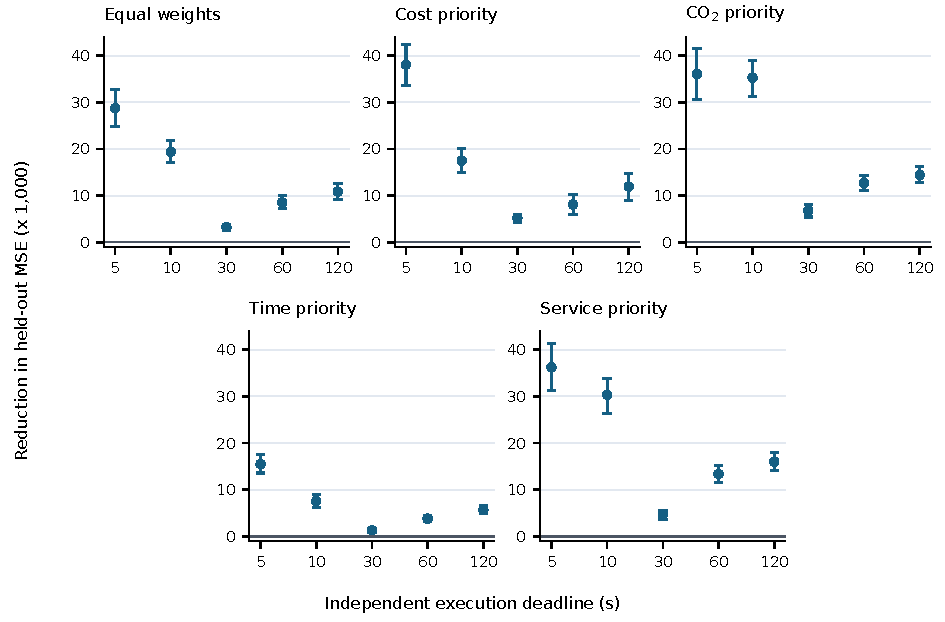
\includegraphics[width=\linewidth]{paper1/results/weights_variants_predictive_gain.pdf}
\caption{Improvement from common to separate deadline-specific coefficient
vectors, by preference and execution deadline. Points and bars show the
estimated MSE reduction and its pointwise 95\% paired-loss bootstrap interval
($10^3$ scale). All 25 intervals lie above zero. Both normalized weights
and coefficient scale are allowed to change; this is not a test of
weight changes alone.}
\label{fig:p1_weight_gains}
\end{figure}

Pooled goodness of fit can conceal serious deadline-specific errors.
For CO$_2$ priority, the common model has pooled $R^2=0.746$, but
$R^2=-0.810$ at 60 seconds and $-1.292$ at 120 seconds. Separate fits
reach 0.710 and 0.647 at those deadlines. The signed common model offers
only small additional gains: its MSE improvement is 0.000338
[0.000169, 0.000501] for Time and 0.000282 [0.000063, 0.000512] for Cost;
the other three intervals contain zero. Relaxing positivity alone is
therefore not the principal improvement observed in these historical fits.
Their linear predictions are not clipped: depending on preference, 13.6--22.9\% of the separate
models' pooled predictions lie outside $[0,1]$. These fits are predictive
comparisons, not calibrated bounded operational scores ready to deploy.
They are retained unchanged; the later projected and fractional-logistic
comparisons are reported separately in Section~\ref{sec:bounded_results}.

\paragraph{A common vector is a preference-dependent compromise.}
Table~\ref{tab:p1_common_weights} reports all 22 component positions.
B1 (zone count) has the largest common point weight in every preference,
from 29.70\% for Cost to 51.46\% for CO$_2$. Its weight interval is
[21.08, 38.15]\% for Cost and [41.17, 69.49]\% for CO$_2$; its bootstrap
rank interval is [1,2] for Cost and [1,1] for the other four preferences.
This is evidence about a size-inclusive score, not an effect beyond size.
Cost assigns 25.78\% [17.58, 34.94] to B3 (estimated binary count),
whereas Time emphasizes B4 (thermal density), 21.08\% [18.19, 23.46],
and A1 (renewable penetration), 10.41\% [5.63, 15.32].

\begin{table}[htbp]\centering\small
\begin{tabular}{lrrrrr}\toprule
Component & Equal & Cost & CO$_2$ & Time & Service\\\midrule
A1 & 2.59 & 4.37 & 0.00 & 10.41 & 0.00\\
A2 & 0.00 & 0.00 & 0.10 & 2.74 & 0.00\\
A3 & 28.48 & 2.64 & 26.53 & 2.17 & 29.16\\
A4 & 0.00 & 0.00 & 0.00 & 0.00 & 0.00\\
A5 & 0.00 & 9.36 & 0.00 & 7.09 & 0.00\\
A6 & 3.95 & 4.02 & 3.24 & 6.04 & 3.38\\
A7 & 0.00 & 0.00 & 0.00 & 6.48 & 0.00\\
A8 & 0.00 & 0.00 & 0.00 & 0.00 & 0.00\\
A9 & 0.00 & 0.00 & 0.00 & 0.00 & 0.00\\
A10 & 0.00 & 0.00 & 0.00 & 0.59 & 0.00\\
A11 & 0.00 & 0.00 & 0.00 & 3.40 & 0.00\\
A12 & 0.00 & 0.00 & 0.00 & 3.83 & 0.00\\
B1 & 45.97 & 29.70 & 51.46 & 33.22 & 46.79\\
B2 & -- & -- & -- & -- & --\\
B3 & 0.00 & 25.78 & 0.00 & 0.00 & 3.11\\
B4 & 14.80 & 13.74 & 10.10 & 21.08 & 10.98\\
B5 & -- & -- & -- & -- & --\\
B6 & 0.00 & 0.00 & 1.89 & 0.00 & 0.00\\
B7 & 0.00 & 0.00 & 0.00 & 0.18 & 0.00\\
B8 & 0.00 & 0.28 & 0.00 & 0.00 & 0.41\\
B9 & 4.21 & 10.09 & 6.68 & 2.77 & 6.17\\
B10 & 0.00 & 0.00 & 0.00 & 0.00 & 0.00\\
\bottomrule\end{tabular}
\caption{Common positive index weights (\%), normalized to sum to 100
before rounding. A1--A12 and B1--B10 follow the order of the component
definitions in Tables~\ref{tab:components} and~\ref{tab:structural_components}. Dashes denote constant B2 and
B5: zero is imposed computationally but is not a learned scientific
weight. Other zeros are boundary estimates under the positivity
constraint, not proof of irrelevance. Intervals for the leading weights are discussed in the text;
individual point ranks do not establish rank separation.}
\label{tab:p1_common_weights}
\end{table}

Large point weights do not always identify individual components.
A3 receives 26.53--29.16\% under Service, Equal and CO$_2$, yet all three
weight intervals include zero. A3 and A5 have correlation 0.99998 and
can exchange weight. B1 and B3 are also strongly correlated (0.9320).
The final common fit selects $\kappa=0$ for Service, Equal and CO$_2$,
and $10^{-4}$ for Time and Cost: regularization does not uniformly
stabilize these estimates. Neither a zero coefficient nor a precise
point ordering should be read as unique physical attribution.

\paragraph{The dominant components change with the deadline.}
Figure~\ref{fig:p1_weight_heatmap} displays all 550 estimated component
weights; Table~\ref{tab:p1_deadline_weights} reports the three largest
at each preference--deadline combination, with their weight intervals.
At 5 seconds, A1 is the largest point weight in all five preferences
(17.6--24.1\%), with regional-connectivity proxy B9, inverse intertie-density proxy A12
or related physical descriptors also prominent. At 10 seconds, B1
leads four preferences (37.6--62.4\%); CO$_2$ instead assigns its largest
weight to B3, 50.4\% [29.1, 64.1]. At 30 seconds, B3 leads all preferences
except Time, for which B1 and B4 receive 37.8\% and 32.7\%.

At 60--120 seconds the preference matters more visibly. Service and Equal
retain large B3, B4 and B9 weights. Time emphasizes B4 together with
B3 and peak-to-firm stress A6; A6 reaches 27.7\% [21.4, 32.6] at
120 seconds. Cost assigns 45.2\% [25.0, 55.5] to B9 at 60 seconds,
compared with 40.8\% [24.5, 55.8] to B3. CO$_2$ assigns 33.3\%
[27.6, 41.6] to B4 and 30.5\% [19.3, 41.8] to B3 at 120 seconds.
These last point-order reversals are not established rank differences:
uncertainty is substantial and the intervals overlap. Figure~\ref{fig:p1_weight_intervals}
shows the uncertainty of the largest point weight in each setting.

\begin{figure}[p]\centering
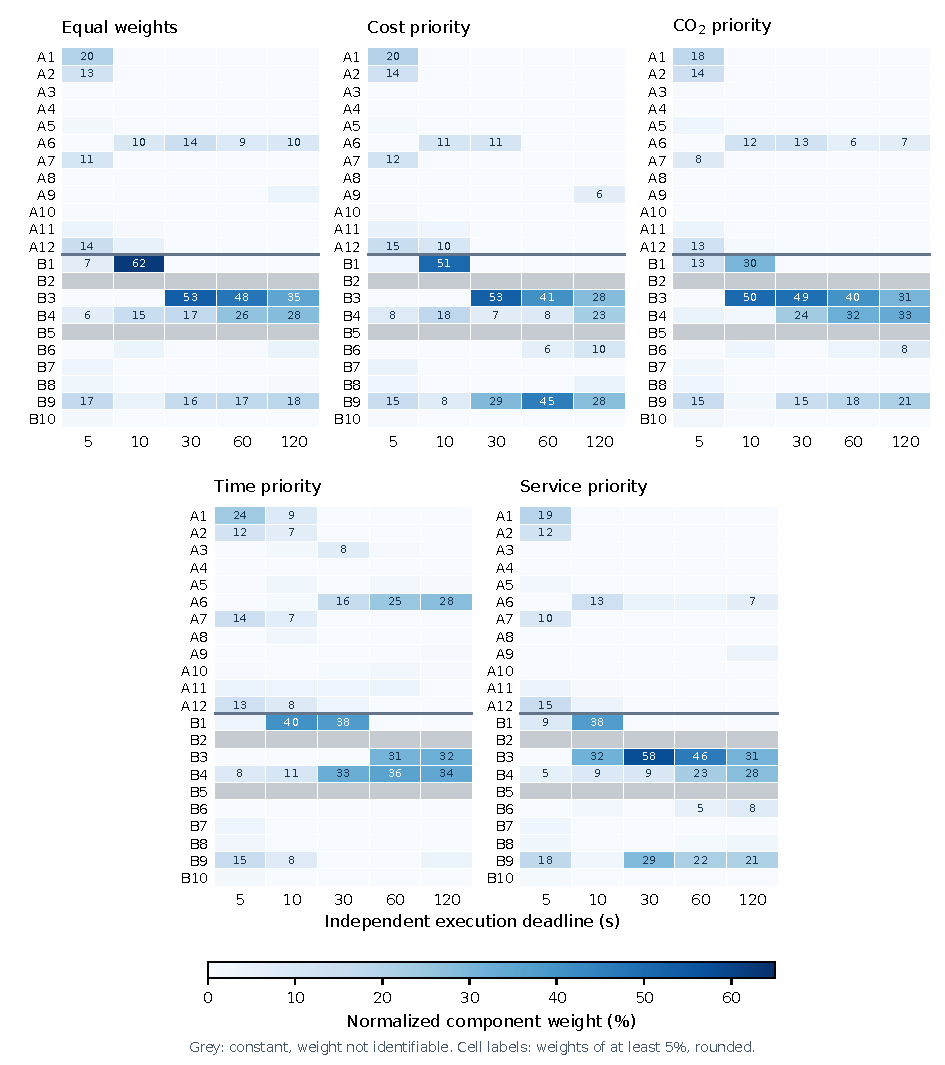
\includegraphics[width=\linewidth]{paper1/results/weights_variants_deadline_heatmap.pdf}
\caption{Normalized positive weights for the 22 criticality components,
five preferences and five independent deadlines. All panels share the
same color scale; cell labels show weights of at least 5\%, rounded to
whole percentages. Gray cells mark constant B2 and B5, whose weights
are not identifiable. Colors represent point estimates, not statistical
significance. Uncertainty for the three leading components is reported
in Table~\ref{tab:p1_deadline_weights}.}
\label{fig:p1_weight_heatmap}
\end{figure}

\begin{table}[p]\centering\footnotesize
\setlength{\tabcolsep}{3pt}
\begin{tabular}{lrlll}\toprule
Preference & $b$ (s) & Largest point weight & Second & Third\\\midrule
Equal & 5 & A1: 20.3 [14.6, 25.9] & B9: 16.5 [10.2, 21.9] & A12: 14.5 [10.5, 17.7]\\
 & 10 & B1: 62.4 [37.6, 71.6] & B4: 15.2 [9.1, 19.5] & A6: 9.6 [4.1, 13.9]\\
 & 30 & B3: 53.1 [38.4, 70.1] & B4: 16.8 [13.1, 20.5] & B9: 15.9 [0.0, 28.4]\\
 & 60 & B3: 47.6 [36.2, 56.7] & B4: 26.3 [21.9, 31.6] & B9: 17.1 [5.0, 23.9]\\
 & 120 & B3: 35.0 [23.9, 48.2] & B4: 28.3 [23.1, 34.5] & B9: 18.3 [6.9, 26.8]\\
\midrule
Cost & 5 & A1: 19.9 [14.7, 25.2] & A12: 15.0 [11.4, 17.8] & B9: 14.9 [8.9, 20.3]\\
 & 10 & B1: 50.6 [37.5, 59.2] & B4: 17.8 [11.6, 23.5] & A6: 10.8 [5.5, 15.6]\\
 & 30 & B3: 53.0 [40.8, 67.5] & B9: 29.1 [16.4, 37.8] & A6: 10.7 [5.2, 15.5]\\
 & 60 & B9: 45.2 [25.0, 55.5] & B3: 40.8 [24.5, 55.8] & B4: 8.1 [4.3, 15.2]\\
 & 120 & B3: 28.3 [15.3, 44.5] & B9: 27.7 [12.1, 40.0] & B4: 22.9 [16.6, 30.8]\\
\midrule
CO$_2$ & 5 & A1: 17.6 [11.4, 23.0] & B9: 14.8 [8.0, 20.3] & A2: 13.9 [9.6, 18.2]\\
 & 10 & B3: 50.4 [29.1, 64.1] & B1: 30.0 [5.5, 42.9] & A6: 12.4 [5.3, 17.7]\\
 & 30 & B3: 49.2 [32.5, 65.6] & B4: 23.5 [19.4, 27.4] & B9: 14.6 [0.0, 29.3]\\
 & 60 & B3: 40.3 [30.4, 50.8] & B4: 32.5 [26.7, 39.2] & B9: 18.2 [6.4, 26.7]\\
 & 120 & B4: 33.3 [27.6, 41.6] & B3: 30.5 [19.3, 41.8] & B9: 21.2 [8.8, 30.5]\\
\midrule
Time & 5 & A1: 24.1 [19.4, 29.6] & B9: 15.0 [9.7, 19.9] & A7: 13.8 [9.1, 18.7]\\
 & 10 & B1: 40.5 [33.6, 46.2] & B4: 10.6 [8.1, 14.0] & A1: 8.7 [3.5, 13.6]\\
 & 30 & B1: 37.8 [27.3, 44.1] & B4: 32.7 [27.5, 35.7] & A6: 15.6 [10.4, 20.8]\\
 & 60 & B4: 35.8 [31.0, 39.8] & B3: 31.0 [17.8, 37.4] & A6: 25.0 [18.8, 29.4]\\
 & 120 & B4: 34.3 [28.7, 39.0] & B3: 32.5 [21.4, 41.7] & A6: 27.7 [21.4, 32.6]\\
\midrule
Service & 5 & A1: 19.1 [13.1, 24.8] & B9: 17.7 [10.9, 23.6] & A12: 14.8 [10.3, 18.1]\\
 & 10 & B1: 37.6 [13.5, 50.0] & B3: 31.6 [16.5, 48.2] & A6: 13.2 [6.5, 17.9]\\
 & 30 & B3: 57.6 [36.4, 78.9] & B9: 28.9 [6.4, 42.1] & B4: 9.4 [5.1, 13.7]\\
 & 60 & B3: 46.1 [33.5, 58.3] & B4: 22.7 [17.8, 30.1] & B9: 21.8 [8.8, 30.0]\\
 & 120 & B3: 30.9 [19.0, 46.2] & B4: 27.8 [22.0, 34.9] & B9: 20.9 [9.2, 30.8]\\
\bottomrule\end{tabular}
\caption{Three largest normalized weights at each deadline, in percent,
with pointwise 95\% scenario-refit bootstrap intervals. The ridge penalty
is fixed during refitting. Components are ordered by the full-cohort
point estimate, not by a statistically established rank. Figure~\ref{fig:p1_weight_heatmap} shows the remaining components. The five deadlines are separate trials.}
\label{tab:p1_deadline_weights}
\end{table}

\begin{figure}[htbp]\centering
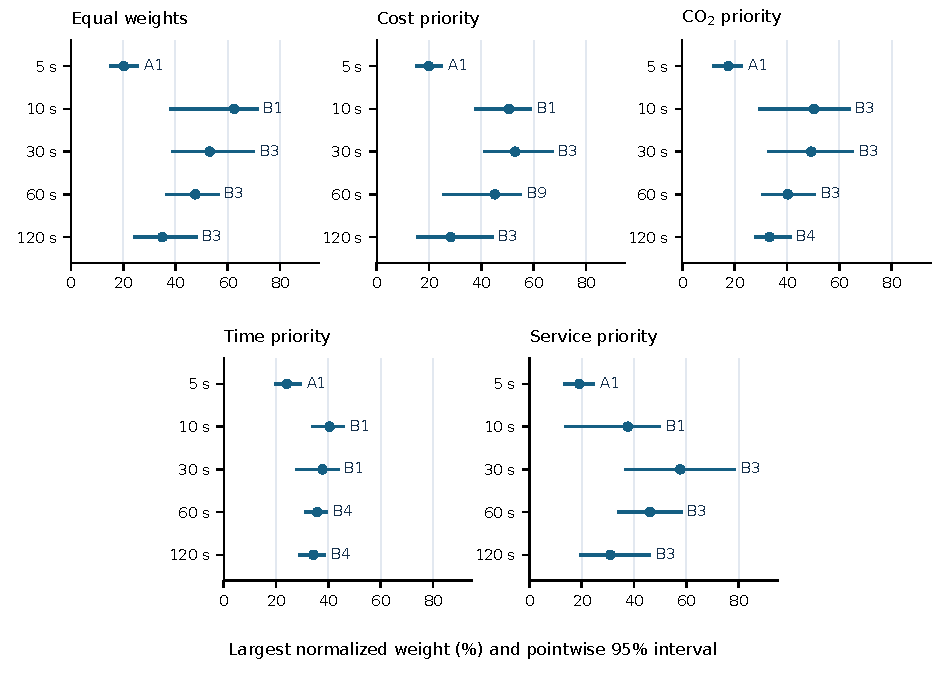
\includegraphics[width=\linewidth]{paper1/results/weights_variants_leading_intervals.pdf}
\caption{Largest point weight at each deadline, with its component ID
and pointwise 95\% interval from 500 scenario refits. The largest
component is selected by its point estimate; the interval is not a
simultaneous or post-selection confidence statement about its rank.
The full three-leading-component comparison is given in
Table~\ref{tab:p1_deadline_weights}.}
\label{fig:p1_weight_intervals}
\end{figure}

These earlier contrasts vary scale and direction together.
The revision's intermediate model in Section~\ref{sec:revision_scale} now
separates those freedoms. Individual weight tables remain conditional
descriptions, not universal physical rankings.


\clearpage
\bibliographystyle{unsrtnat}\bibliography{paper1/references}
\end{document}
